% Options for packages loaded elsewhere
\PassOptionsToPackage{unicode}{hyperref}
\PassOptionsToPackage{hyphens}{url}
\documentclass[
]{book}
\usepackage{xcolor}
\usepackage{amsmath,amssymb}
\setcounter{secnumdepth}{-\maxdimen} % remove section numbering
\usepackage{iftex}
\ifPDFTeX
  \usepackage[T1]{fontenc}
  \usepackage[utf8]{inputenc}
  \usepackage{textcomp} % provide euro and other symbols
\else % if luatex or xetex
  \usepackage{unicode-math} % this also loads fontspec
  \defaultfontfeatures{Scale=MatchLowercase}
  \defaultfontfeatures[\rmfamily]{Ligatures=TeX,Scale=1}
\fi
\usepackage{lmodern}
\ifPDFTeX\else
  % xetex/luatex font selection
\fi
% Use upquote if available, for straight quotes in verbatim environments
\IfFileExists{upquote.sty}{\usepackage{upquote}}{}
\IfFileExists{microtype.sty}{% use microtype if available
  \usepackage[]{microtype}
  \UseMicrotypeSet[protrusion]{basicmath} % disable protrusion for tt fonts
}{}
\makeatletter
\@ifundefined{KOMAClassName}{% if non-KOMA class
  \IfFileExists{parskip.sty}{%
    \usepackage{parskip}
  }{% else
    \setlength{\parindent}{0pt}
    \setlength{\parskip}{6pt plus 2pt minus 1pt}}
}{% if KOMA class
  \KOMAoptions{parskip=half}}
\makeatother
\usepackage{graphicx}
\makeatletter
\newsavebox\pandoc@box
\newcommand*\pandocbounded[1]{% scales image to fit in text height/width
  \sbox\pandoc@box{#1}%
  \Gscale@div\@tempa{\textheight}{\dimexpr\ht\pandoc@box+\dp\pandoc@box\relax}%
  \Gscale@div\@tempb{\linewidth}{\wd\pandoc@box}%
  \ifdim\@tempb\p@<\@tempa\p@\let\@tempa\@tempb\fi% select the smaller of both
  \ifdim\@tempa\p@<\p@\scalebox{\@tempa}{\usebox\pandoc@box}%
  \else\usebox{\pandoc@box}%
  \fi%
}
% Set default figure placement to htbp
\def\fps@figure{htbp}
\makeatother
\setlength{\emergencystretch}{3em} % prevent overfull lines
\providecommand{\tightlist}{%
  \setlength{\itemsep}{0pt}\setlength{\parskip}{0pt}}
\usepackage{bookmark}
\IfFileExists{xurl.sty}{\usepackage{xurl}}{} % add URL line breaks if available
\urlstyle{same}
\hypersetup{
  hidelinks,
  pdfcreator={LaTeX via pandoc}}

\author{}
\date{}

\begin{document}
\frontmatter

\mainmatter
\chapter{EMT untuk Statistika}\label{emt-untuk-statistika}

Dalam buku catatan ini, kita mendemonstrasikan plot statistik utama, tes, dan distribusi dalam Euler.

Mari kita mulai dengan beberapa statistik deskriptif. Ini bukanlah sebuah pengantar statistik. Jadi, mungkin memerlukan latar belakang untuk memahami detailnya.

Asumsikan pengukuran-pengukuran berikut ini. Kita ingin menghitung nilai rata-rata dan deviasi standar yang diukur.

\textgreater M={[}1000,1004,998,997,1002,1001,998,1004,998,997{]}; \ldots{}\\
\textgreater{} median(M), mean(M), dev(M),

\begin{verbatim}
999
999.9
2.72641400622
\end{verbatim}

Kita dapat memplot plot kotak dan kumis untuk data tersebut. Dalam kasus kami, tidak ada pencilan.

\textgreater aspect(1.75); boxplot(M):

\begin{figure}
\centering
\pandocbounded{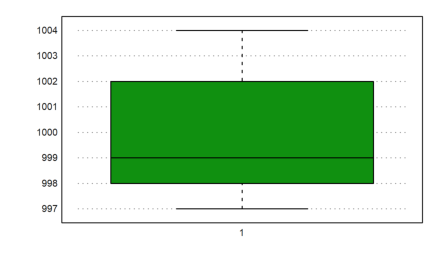
\includegraphics[keepaspectratio]{images/EMT4Statistika - Naila Khalidatus Salwa-001.png}}
\caption{images/EMT4Statistika\%20-\%20Naila\%20Khalidatus\%20Salwa-001.png}
\end{figure}

Boxplot(M) digunakan untuk membuat boxplot atau diagram kotak dari data di dalam variabel M. Boxplot adalah visualisasi statistik yang menunjukkan persebaran data, termasuk nilai minimum, median, dan nilai maksimum.

Kami menghitung probabilitas bahwa suatu nilai lebih besar dari 1005, dengan mengasumsikan nilai yang diukur dari distribusi normal.

Semua fungsi untuk distribusi dalam Euler diakhiri dengan \ldots dis dan menghitung distribusi probabilitas kumulatif (CPF).

\[\text{normaldis(x,m,d)}=\int_{-\infty}^x \frac{1}{d\sqrt{2\pi}}e^{-\frac{1}{2}(\frac{t-m}{d})^2}\ dt.\]Kami mencetak hasilnya dalam \% dengan akurasi 2 digit menggunakan fungsi cetak.

\textgreater print((1-normaldis(1005,mean(M),dev(M)))*100,2,unit='' \%``)

\begin{verbatim}
      3.07 %
\end{verbatim}

Untuk contoh berikutnya, kami mengasumsikan jumlah pria berikut dalam rentang ukuran tertentu.

\textgreater r=155.5:4:187.5; v={[}22,71,136,169,139,71,32,8{]};

Berikut ini adalah plot distribusi.

\textgreater plot2d(r,v,a=150,b=200,c=0,d=190,bar=1,style=``\textbackslash/''):

\begin{figure}
\centering
\pandocbounded{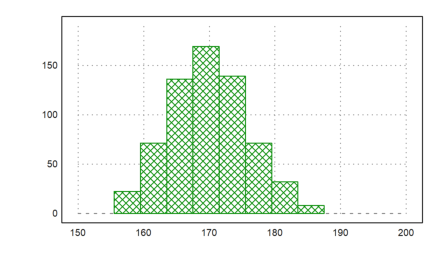
\includegraphics[keepaspectratio]{images/EMT4Statistika - Naila Khalidatus Salwa-003.png}}
\caption{images/EMT4Statistika\%20-\%20Naila\%20Khalidatus\%20Salwa-003.png}
\end{figure}

Kita dapat memasukkan data mentah tersebut ke dalam tabel.

Tabel adalah sebuah metode untuk menyimpan data statistik. Tabel kita harus berisi tiga kolom: Awal rentang, akhir rentang, jumlah orang dalam rentang.

Tabel dapat dicetak dengan header. Kami menggunakan vektor string untuk mengatur header.

\textgreater T:=r{[}1:8{]}' \textbar{} r{[}2:9{]}' \textbar{} v'; writetable(T,labc={[}``BB'',``BA'',``Frek''{]})

\begin{verbatim}
        BB        BA      Frek
     155.5     159.5        22
     159.5     163.5        71
     163.5     167.5       136
     167.5     171.5       169
     171.5     175.5       139
     175.5     179.5        71
     179.5     183.5        32
     183.5     187.5         8
\end{verbatim}

Jika kita membutuhkan nilai rata-rata dan statistik lain dari ukuran, kita perlu menghitung titik tengah rentang. Kita dapat menggunakan dua kolom pertama dari tabel kita untuk ini.

Simbol ``\textbar{}'' digunakan untuk memisahkan kolom, fungsi ``writetable'' digunakan untuk menulis tabel, dengan opsi ``labc'' untuk menentukan judul kolom.

\textgreater(T{[},1{]}+T{[},2{]})/2 // the midpoint of each interval

\begin{verbatim}
        157.5 
        161.5 
        165.5 
        169.5 
        173.5 
        177.5 
        181.5 
        185.5 
\end{verbatim}

Tetapi akan lebih mudah, untuk melipat rentang dengan vektor {[}1/2,1/2{]}.

\textgreater M=fold(r,{[}0.5,0.5{]})

\begin{verbatim}
[157.5,  161.5,  165.5,  169.5,  173.5,  177.5,  181.5,  185.5]
\end{verbatim}

Sekarang kita dapat menghitung rata-rata dan deviasi sampel dengan frekuensi yang diberikan.

\textgreater\{m,d\}=meandev(M,v); m, d,

\begin{verbatim}
169.901234568
5.98912964449
\end{verbatim}

Mari kita tambahkan distribusi normal dari nilai-nilai tersebut ke dalam diagram batang di atas. Rumus untuk distribusi normal dengan rata-rata m dan deviasi standar d adalah:

\[y=\frac{1}{d\sqrt{2\pi}}e^{\frac{-(x-m)^2}{2d^2}}.\]Karena nilainya antara 0 dan 1, untuk memplotnya pada plot batang, maka harus dikalikan dengan 4 kali jumlah data.

\textgreater plot2d(``qnormal(x,m,d)*sum(v)*4'', \ldots{}\\
\textgreater{} xmin=min(r),xmax=max(r),thickness=3,add=1):

\begin{figure}
\centering
\pandocbounded{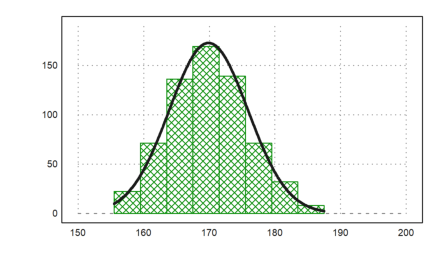
\includegraphics[keepaspectratio]{images/EMT4Statistika - Naila Khalidatus Salwa-005.png}}
\caption{images/EMT4Statistika\%20-\%20Naila\%20Khalidatus\%20Salwa-005.png}
\end{figure}

\chapter{Tabel}\label{tabel}

Dalam direktori buku catatan ini, kita akan menemukan file dengan tabel. Data tersebut mewakili hasil survei. Berikut adalah empat baris pertama dari file tersebut. Data berasal dari sebuah buku online berbahasa Jerman ``Einführung in die Statistik mit R'' oleh A. Handl.

\textgreater printfile(``table.dat'',4);

\begin{verbatim}
Person Sex Age Titanic Evaluation Tip Problem
1 m 30 n . 1.80 n
2 f 23 y g 1.80 n
3 f 26 y g 1.80 y
\end{verbatim}

Tabel berisi 7 kolom angka atau token (string). Kita ingin membaca tabel tersebut dari file. Pertama, kita menggunakan terjemahan kita sendiri untuk token-token tersebut.

Untuk itu, kita mendefinisikan set token. Fungsi strtokens() mendapatkan vektor string token dari string yang diberikan.

\textgreater mf:={[}``m'',``f''{]}; yn:={[}``y'',``n''{]}; ev:=strtokens(``g vg m b vb'');

Sekarang kita membaca tabel dengan terjemahan ini.

Argumen tok2, tok4, dan seterusnya adalah terjemahan dari kolom-kolom pada tabel. Argumen-argumen ini tidak ada dalam daftar parameter readtable(), jadi Anda perlu memberikannya dengan ``:=''.

\textgreater\{MT,hd\}=readtable(``table.dat'',tok2:=mf,tok4:=yn,tok5:=ev,tok7:=yn);

\textgreater load over statistics;

Untuk mencetak, kita perlu menentukan set token yang sama. Kami mencetak empat baris pertama saja.

\textgreater writetable(MT{[}1:10{]},labc=hd,wc=5,tok2:=mf,tok4:=yn,tok5:=ev,tok7:=yn);

\begin{verbatim}
 Person  Sex  Age Titanic Evaluation  Tip Problem
      1    m   30       n          .  1.8       n
      2    f   23       y          g  1.8       n
      3    f   26       y          g  1.8       y
      4    m   33       n          .  2.8       n
      5    m   37       n          .  1.8       n
      6    m   28       y          g  2.8       y
      7    f   31       y         vg  2.8       n
      8    m   23       n          .  0.8       n
      9    f   24       y         vg  1.8       y
     10    m   26       n          .  1.8       n
\end{verbatim}

Titik-titik ``.'' mewakili nilai yang tidak tersedia.

Jika kita tidak ingin menentukan token untuk terjemahan sebelumnya, kita hanya perlu menentukan kolom mana yang berisi token dan bukan angka.

\textgreater ctok={[}2,4,5,7{]}; \{MT,hd,tok\}=readtable(``table.dat'',ctok=ctok);

Fungsi readtable() sekarang mengembalikan satu set token.

\textgreater tok

\begin{verbatim}
m
n
f
y
g
vg
\end{verbatim}

Tabel berisi entri dari file dengan token yang diterjemahkan menjadi angka.

String khusus NA=``.'' ditafsirkan sebagai ``Tidak Tersedia'', dan mendapatkan NAN (bukan angka) dalam tabel. Terjemahan ini dapat diubah dengan parameter NA, dan NAval.

\textgreater MT{[}1{]}

\begin{verbatim}
[1,  1,  30,  2,  NAN,  1.8,  2]
\end{verbatim}

Berikut ini adalah isi tabel dengan angka yang tidak diterjemahkan.

\textgreater writetable(MT,wc=5)

\begin{verbatim}
    1    1   30    2    .  1.8    2
    2    3   23    4    5  1.8    2
    3    3   26    4    5  1.8    4
    4    1   33    2    .  2.8    2
    5    1   37    2    .  1.8    2
    6    1   28    4    5  2.8    4
    7    3   31    4    6  2.8    2
    8    1   23    2    .  0.8    2
    9    3   24    4    6  1.8    4
   10    1   26    2    .  1.8    2
   11    3   23    4    6  1.8    4
   12    1   32    4    5  1.8    2
   13    1   29    4    6  1.8    4
   14    3   25    4    5  1.8    4
   15    3   31    4    5  0.8    2
   16    1   26    4    5  2.8    2
   17    1   37    2    .  3.8    2
   18    1   38    4    5    .    2
   19    3   29    2    .  3.8    2
   20    3   28    4    6  1.8    2
   21    3   28    4    1  2.8    4
   22    3   28    4    6  1.8    4
   23    3   38    4    5  2.8    2
   24    3   27    4    1  1.8    4
   25    1   27    2    .  2.8    4
\end{verbatim}

Untuk kenyamanan, Anda dapat meletakkan output dari readtable() ke dalam sebuah daftar.

\textgreater Table=\{\{readtable(``table.dat'',ctok=ctok)\}\};

Dengan menggunakan kolom token yang sama dan token yang dibaca dari file, kita dapat mencetak tabel. Kita dapat menentukan ctok, tok, dll. atau menggunakan daftar Tabel.

\textgreater writetable(Table,ctok=ctok,wc=5);

\begin{verbatim}
 Person  Sex  Age Titanic Evaluation  Tip Problem
      1    m   30       n          .  1.8       n
      2    f   23       y          g  1.8       n
      3    f   26       y          g  1.8       y
      4    m   33       n          .  2.8       n
      5    m   37       n          .  1.8       n
      6    m   28       y          g  2.8       y
      7    f   31       y         vg  2.8       n
      8    m   23       n          .  0.8       n
      9    f   24       y         vg  1.8       y
     10    m   26       n          .  1.8       n
     11    f   23       y         vg  1.8       y
     12    m   32       y          g  1.8       n
     13    m   29       y         vg  1.8       y
     14    f   25       y          g  1.8       y
     15    f   31       y          g  0.8       n
     16    m   26       y          g  2.8       n
     17    m   37       n          .  3.8       n
     18    m   38       y          g    .       n
     19    f   29       n          .  3.8       n
     20    f   28       y         vg  1.8       n
     21    f   28       y          m  2.8       y
     22    f   28       y         vg  1.8       y
     23    f   38       y          g  2.8       n
     24    f   27       y          m  1.8       y
     25    m   27       n          .  2.8       y
\end{verbatim}

Fungsi tablecol() mengembalikan nilai kolom dari tabel, melewatkan setiap baris dengan nilai NAN (``.'' dalam file), dan indeks kolom, yang berisi nilai-nilai ini.

\textgreater\{c,i\}=tablecol(MT,{[}5,6{]});

Kita dapat menggunakan ini untuk mengekstrak kolom dari tabel untuk tabel baru.

\textgreater j={[}1,5,6{]}; writetable(MT{[}i,j{]},labc=hd{[}j{]},ctok={[}2{]},tok=tok)

\begin{verbatim}
    Person Evaluation       Tip
         2          g       1.8
         3          g       1.8
         6          g       2.8
         7         vg       2.8
         9         vg       1.8
        11         vg       1.8
        12          g       1.8
        13         vg       1.8
        14          g       1.8
        15          g       0.8
        16          g       2.8
        20         vg       1.8
        21          m       2.8
        22         vg       1.8
        23          g       2.8
        24          m       1.8
\end{verbatim}

Tentu saja, kita perlu mengekstrak tabel itu sendiri dari daftar Tabel dalam kasus ini.

\textgreater MT=Table{[}1{]};

Tentu saja, kita juga dapat menggunakannya untuk menentukan nilai rata-rata kolom atau nilai statistik lainnya.

\textgreater mean(tablecol(MT,6))

\begin{verbatim}
2.175
\end{verbatim}

Fungsi getstatistics() mengembalikan elemen-elemen dalam sebuah vektor, dan jumlahnya. Kita menerapkannya pada nilai ``m'' dan ``f'' pada kolom kedua tabel kita.

\textgreater\{xu,count\}=getstatistics(tablecol(MT,2)); xu, count,

\begin{verbatim}
[1,  3]
[12,  13]
\end{verbatim}

Kita bisa mencetak hasilnya dalam tabel baru.

\textgreater writetable(count',labr=tok{[}xu{]})

\begin{verbatim}
         m        12
         f        13
\end{verbatim}

Fungsi selecttable() mengembalikan tabel baru dengan nilai dalam satu kolom yang dipilih dari vektor indeks. Pertama, kita mencari indeks dari dua nilai kita dalam tabel token.

\textgreater v:=indexof(tok,{[}``g'',``vg''{]})

\begin{verbatim}
[5,  6]
\end{verbatim}

Sekarang kita dapat memilih baris dari tabel, yang memiliki salah satu nilai dalam v di baris ke-5.

\textgreater MT1:=MT{[}selectrows(MT,5,v){]}; i:=sortedrows(MT1,5);

Sekarang kita dapat mencetak tabel, dengan nilai yang diekstrak dan diurutkan di kolom ke-5.

\textgreater writetable(MT1{[}i{]},labc=hd,ctok=ctok,tok=tok,wc=7);

\begin{verbatim}
 Person    Sex    Age Titanic Evaluation    Tip Problem
      2      f     23       y          g    1.8       n
      3      f     26       y          g    1.8       y
      6      m     28       y          g    2.8       y
     18      m     38       y          g      .       n
     16      m     26       y          g    2.8       n
     15      f     31       y          g    0.8       n
     12      m     32       y          g    1.8       n
     23      f     38       y          g    2.8       n
     14      f     25       y          g    1.8       y
      9      f     24       y         vg    1.8       y
      7      f     31       y         vg    2.8       n
     20      f     28       y         vg    1.8       n
     22      f     28       y         vg    1.8       y
     13      m     29       y         vg    1.8       y
     11      f     23       y         vg    1.8       y
\end{verbatim}

Untuk statistik berikutnya, kita ingin menghubungkan dua kolom tabel. Jadi kita mengekstrak kolom 2 dan 4 dan mengurutkan tabel.

\textgreater i=sortedrows(MT,{[}2,4{]}); \ldots{}\\
\textgreater{} writetable(tablecol(MT{[}i{]},{[}2,4{]})',ctok={[}1,2{]},tok=tok)

\begin{verbatim}
         m         n
         m         n
         m         n
         m         n
         m         n
         m         n
         m         n
         m         y
         m         y
         m         y
         m         y
         m         y
         f         n
         f         y
         f         y
         f         y
         f         y
         f         y
         f         y
         f         y
         f         y
         f         y
         f         y
         f         y
         f         y
\end{verbatim}

Dengan getstatistics(), kita juga dapat menghubungkan hitungan dalam dua kolom tabel satu sama lain.

\textgreater MT24=tablecol(MT,{[}2,4{]}); \ldots{}\\
\textgreater{} \{xu1,xu2,count\}=getstatistics(MT24{[}1{]},MT24{[}2{]}); \ldots{}\\
\textgreater{} writetable(count,labr=tok{[}xu1{]},labc=tok{[}xu2{]})

\begin{verbatim}
                   n         y
         m         7         5
         f         1        12
\end{verbatim}

Tabel dapat ditulis ke sebuah file.

\textgreater filename=``test.dat''; \ldots{}\\
\textgreater{} writetable(count,labr=tok{[}xu1{]},labc=tok{[}xu2{]},file=filename);

Kemudian kita dapat membaca tabel dari file tersebut.

\textgreater\{MT2,hd,tok2,hdr\}=readtable(filename,\textgreater clabs,\textgreater rlabs); \ldots{}\\
\textgreater{} writetable(MT2,labr=hdr,labc=hd)

\begin{verbatim}
                   n         y
         m         7         5
         f         1        12
\end{verbatim}

Dan hapus file tersebut.

\textgreater fileremove(filename);

\chapter{Distribusi}\label{distribusi}

Dengan plot2d, ada metode yang sangat mudah untuk memplot distribusi data eksperimen.

\textgreater p=normal(1,1000); //1000 random normal-distributed sample p

\textgreater plot2d(p,distribution=20,style=``\textbackslash/''); // plot the random sample p

\textgreater plot2d(``qnormal(x,0,1)'',add=1): // add the standard normal distribution plot

\begin{figure}
\centering
\pandocbounded{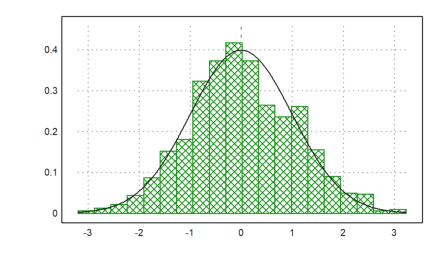
\includegraphics[keepaspectratio]{images/EMT4Statistika - Naila Khalidatus Salwa-006.png}}
\caption{images/EMT4Statistika\%20-\%20Naila\%20Khalidatus\%20Salwa-006.png}
\end{figure}

Harap perhatikan perbedaan antara plot batang (sampel) dan kurva normal (distribusi nyata). Masukkan kembali ketiga perintah tersebut untuk melihat hasil pengambilan sampel yang lain.

Berikut ini adalah perbandingan 10 simulasi dari 1000 nilai terdistribusi normal dengan menggunakan apa yang disebut box plot. Plot ini menunjukkan median, kuartil 25\% dan 75\%, nilai minimal dan maksimal, serta pencilan.

\textgreater p=normal(10,1000); boxplot(p):

\begin{figure}
\centering
\pandocbounded{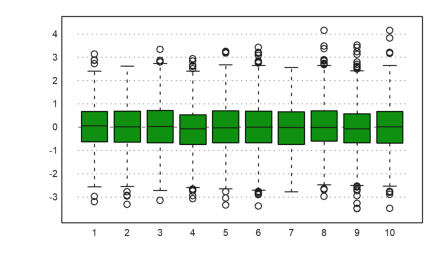
\includegraphics[keepaspectratio]{images/EMT4Statistika - Naila Khalidatus Salwa-007.png}}
\caption{images/EMT4Statistika\%20-\%20Naila\%20Khalidatus\%20Salwa-007.png}
\end{figure}

Untuk menghasilkan bilangan bulat acak, Euler memiliki intrandom. Mari kita simulasikan pelemparan dadu dan plot distribusinya.

Kita menggunakan fungsi getmultiplicities(v,x), yang menghitung seberapa sering elemen-elemen dari v muncul di dalam x. Kemudian kita memplot hasilnya menggunakan columnsplot().

\textgreater k=intrandom(1,6000,6); \ldots{}\\
\textgreater{} columnsplot(getmultiplicities(1:6,k)); \ldots{}\\
\textgreater{} ygrid(1000,color=red):

\begin{figure}
\centering
\pandocbounded{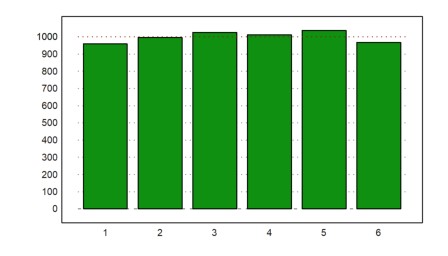
\includegraphics[keepaspectratio]{images/EMT4Statistika - Naila Khalidatus Salwa-008.png}}
\caption{images/EMT4Statistika\%20-\%20Naila\%20Khalidatus\%20Salwa-008.png}
\end{figure}

Walaupun intrandom(n,m,k) mengembalikan bilangan bulat yang terdistribusi secara seragam dari 1 sampai k, adalah mungkin untuk menggunakan distribusi bilangan bulat yang lain dengan randpint().

Pada contoh berikut, probabilitas untuk 1,2,3 adalah 0.4, 0.1, 0.5 secara berurutan.

\textgreater randpint(1,1000,{[}0.4,0.1,0.5{]}); getmultiplicities(1:3,\%)

\begin{verbatim}
[401,  106,  493]
\end{verbatim}

Euler dapat menghasilkan nilai acak dari lebih banyak distribusi. Lihatlah ke dalam referensi.

Misalnya, kita mencoba distribusi eksponensial. Sebuah variabel acak kontinu X dikatakan memiliki distribusi eksponensial, jika PDF-nya diberikan oleh

\[f_X(x)=\lambda e^{-\lambda x},\quad x>0,\quad \lambda>0,\]dengan parameter

\[\lambda=\frac{1}{\mu},\quad \mu \text{ adalah rata-rata, dan dilambangkan dengan} X \sim \text{Exponential}(\lambda).\]\textgreater plot2d(randexponential(1,1000,2),\textgreater distribution):

\begin{figure}
\centering
\pandocbounded{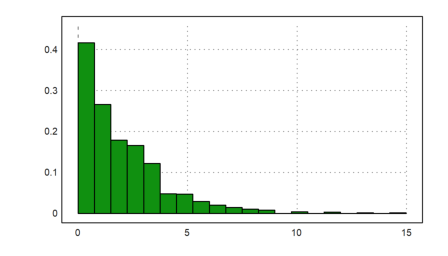
\includegraphics[keepaspectratio]{images/EMT4Statistika - Naila Khalidatus Salwa-011.png}}
\caption{images/EMT4Statistika\%20-\%20Naila\%20Khalidatus\%20Salwa-011.png}
\end{figure}

Untuk banyak distribusi, Euler dapat menghitung fungsi distribusi dan kebalikannya.

\textgreater plot2d(``normaldis'',-4,4):

\begin{figure}
\centering
\pandocbounded{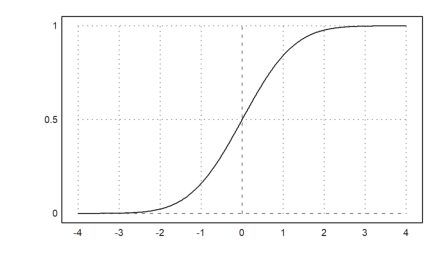
\includegraphics[keepaspectratio]{images/EMT4Statistika - Naila Khalidatus Salwa-012.png}}
\caption{images/EMT4Statistika\%20-\%20Naila\%20Khalidatus\%20Salwa-012.png}
\end{figure}

Berikut ini adalah salah satu cara untuk memplot kuantil.

\textgreater plot2d(``qnormal(x,1,1.5)'',-4,6); \ldots{}\\
\textgreater{} plot2d(``qnormal(x,1,1.5)'',a=2,b=5,\textgreater add,\textgreater filled):

\begin{figure}
\centering
\pandocbounded{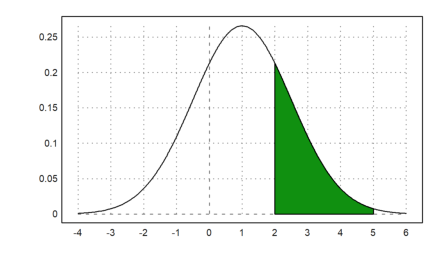
\includegraphics[keepaspectratio]{images/EMT4Statistika - Naila Khalidatus Salwa-013.png}}
\caption{images/EMT4Statistika\%20-\%20Naila\%20Khalidatus\%20Salwa-013.png}
\end{figure}

\[\text{normaldis(x,m,d)}=\int_{-\infty}^x \frac{1}{d\sqrt{2\pi}}e^{-\frac{1}{2}(\frac{t-m}{d})^2}\ dt.\]

Probabilitas untuk berada di area hijau adalah sebagai berikut.

\textgreater normaldis(5,1,1.5)-normaldis(2,1,1.5)

\begin{verbatim}
0.248662156979
\end{verbatim}

Hal ini dapat dihitung secara numerik dengan integral berikut ini.

\[\int_2^5 \frac{1}{1.5\sqrt{2\pi}}e^{-\frac{1}{2}(\frac{x-1}{1.5})^2}\ dx.\]\textgreater gauss(``qnormal(x,1,1.5)'',2,5)

\begin{verbatim}
0.248662156979
\end{verbatim}

Mari kita bandingkan distribusi binomial dengan distribusi normal dengan rata-rata dan deviasi yang sama. Fungsi invbindis() menyelesaikan interpolasi linier antara nilai bilangan bulat.

\textgreater invbindis(0.95,1000,0.5), invnormaldis(0.95,500,0.5*sqrt(1000))

\begin{verbatim}
525.516721219
526.007419394
\end{verbatim}

Fungsi qdis() adalah densitas dari distribusi chi-square. Seperti biasa, Euler memetakan vektor ke fungsi ini. Dengan demikian kita mendapatkan plot semua distribusi chi-kuadrat dengan derajat 5 hingga 30 dengan mudah dengan cara berikut.

\textgreater plot2d(``qchidis(x,(5:5:50)')'',0,50):

\begin{figure}
\centering
\pandocbounded{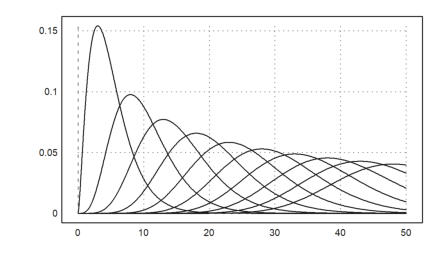
\includegraphics[keepaspectratio]{images/EMT4Statistika - Naila Khalidatus Salwa-016.png}}
\caption{images/EMT4Statistika\%20-\%20Naila\%20Khalidatus\%20Salwa-016.png}
\end{figure}

Euler memiliki fungsi-fungsi yang akurat untuk mengevaluasi distribusi-distribusi. Mari kita periksa chidis() dengan sebuah integral.

Penamaannya diusahakan agar konsisten. Contohnya,

\begin{itemize}
\item
  distribusi chi-square adalah chidis(),
\item
  fungsi invers adalah invchidis(),
\item
  densitasnya adalah qchidis().
\end{itemize}

Pelengkap dari distribusi (ekor atas) adalah chicdis().

\textgreater chidis(1.5,2), integrate(``qchidis(x,2)'',0,1.5)

\begin{verbatim}
0.527633447259
0.527633447259
\end{verbatim}

\chapter{Distribusi Diskrit}\label{distribusi-diskrit}

Distribusi diskrit adalah jenis distribusi probablitas yang digunakan untuk variabel acak diskrit, yaitu variabel yang hanya dapat memiliki nilai tertentu, biasanya dalam bentuk bilangan bulat.

Untuk menentukan distribusi diskrit Anda sendiri, Anda dapat menggunakan metode berikut.

Pertama, kita tetapkan fungsi distribusinya.

\textgreater wd = 0\textbar((1:6)+{[}-0.01,0.01,0,0,0,0{]})/6

\begin{verbatim}
[0,  0.165,  0.335,  0.5,  0.666667,  0.833333,  1]
\end{verbatim}

Artinya, dengan probabilitas wd{[}i+1{]}-wd{[}i{]} kita menghasilkan nilai acak i.

Ini adalah distribusi yang hampir seragam. Mari kita tentukan sebuah generator angka acak untuk ini. Fungsi find(v,x) menemukan nilai x dalam vektor v. Fungsi ini juga dapat digunakan untuk vektor x.

\textgreater function wrongdice (n,m) := find(wd,random(n,m))

Kesalahan ini sangat halus sehingga kita hanya bisa melihatnya setelah melakukan iterasi yang sangat banyak.

Fungsi wrongdice mengembalikan sebuah matriks berukuran n x m, di mana setiap elemen dari matriks ini adalah indeks posisi dari elemen wd yang paling sesuai (atau mendekati) niali acak dari random (n, m).

\textgreater columnsplot(getmultiplicities(1:6,wrongdice(1,1000000))):

\begin{figure}
\centering
\pandocbounded{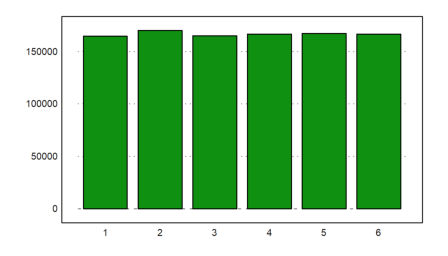
\includegraphics[keepaspectratio]{images/EMT4Statistika - Naila Khalidatus Salwa-017.png}}
\caption{images/EMT4Statistika\%20-\%20Naila\%20Khalidatus\%20Salwa-017.png}
\end{figure}

Berikut ini adalah fungsi sederhana untuk memeriksa distribusi seragam dari nilai 1\ldots{} K dalam v. Kami menerima hasilnya, jika untuk semua frekuensi

\[\left|f_i-\frac{1}{K}\right| < \frac{\delta}{\sqrt{n}}.\]\textgreater function checkrandom (v, delta=1) \ldots{}

\begin{verbatim}
  K=max(v); n=cols(v);
  fr=getfrequencies(v,1:K);
  return max(fr/n-1/K)<delta/sqrt(n);
  endfunction
\end{verbatim}

Memang fungsi ini menolak distribusi seragam.

\textgreater checkrandom(wrongdice(1,1000000))

\begin{verbatim}
0
\end{verbatim}

Dan ini menerima generator acak bawaan.

\textgreater checkrandom(intrandom(1,1000000,6))

\begin{verbatim}
1
\end{verbatim}

Checkrandom mengembalikan 1 atau true yang berarti bahwa distribusi dari 1 juta bilangan acak rentang 1 sampai 6 dianggap cukup seragam dalam batas toleransi yang ditetapkan.

Kita dapat menghitung distribusi binomial. Pertama, ada binomialsum(), yang mengembalikan probabilitas i atau kurang dari n percobaan.

\textgreater bindis(410,1000,0.4)

\begin{verbatim}
0.751401349654
\end{verbatim}

Fungsi Beta terbalik digunakan untuk menghitung interval kepercayaan Clopper-Pearson untuk parameter p.~Tingkat defaultnya adalah alpha.

Arti dari interval ini adalah jika p berada di luar interval, hasil yang diamati sebesar 410 dalam 1000 jarang terjadi.

\textgreater clopperpearson(410,1000)

\begin{verbatim}
[0.37932,  0.441212]
\end{verbatim}

Perintah berikut ini adalah cara langsung untuk mendapatkan hasil di atas. Tetapi untuk n yang besar, penjumlahan langsung tidak akurat dan lambat.

\textgreater p=0.4; i=0:410; n=1000; sum(bin(n,i)*p\textsuperscript{i*(1-p)}(n-i))

\begin{verbatim}
0.751401349655
\end{verbatim}

Omong-omong, invbinsum() menghitung kebalikan dari binomialsum().

\textgreater invbindis(0.75,1000,0.4)

\begin{verbatim}
409.932733047
\end{verbatim}

Dalam Bridge, kami mengasumsikan 5 kartu yang beredar (dari 52 kartu) di dua tangan (26 kartu). Mari kita hitung probabilitas distribusi yang lebih buruk dari 3:2 (misalnya 0:5, 1:4, 4:1, atau 5:0).

\textgreater2*hypergeomsum(1,5,13,26)

\begin{verbatim}
0.321739130435
\end{verbatim}

Ada juga simulasi distribusi multinomial.

\textgreater randmultinomial(10,1000,{[}0.4,0.1,0.5{]})

\begin{verbatim}
          394            82           524 
          418            92           490 
          445            90           465 
          403           114           483 
          405            95           500 
          384           107           509 
          414            93           493 
          419            90           491 
          394           101           505 
          382           103           515 
\end{verbatim}

\chapter{Memplot Data}\label{memplot-data}

Untuk memplot data, kita mencoba menggunakan hasil pemilihan umum Jerman sejak tahun 1990, yang diukur dalam kursi.

\textgreater BW := {[} \ldots{}\\
\textgreater{} 1990,662,319,239,79,8,17; \ldots{}\\
\textgreater{} 1994,672,294,252,47,49,30; \ldots{}\\
\textgreater{} 1998,669,245,298,43,47,36; \ldots{}\\
\textgreater{} 2002,603,248,251,47,55,2; \ldots{}\\
\textgreater{} 2005,614,226,222,61,51,54; \ldots{}\\
\textgreater{} 2009,622,239,146,93,68,76; \ldots{}\\
\textgreater{} 2013,631,311,193,0,63,64{]};

Untuk beberapa bagian, menggunakan serangkaian nama.

\textgreater P:={[}``CDU/CSU'',``SPD'',``FDP'',``Gr'',``Li''{]};

Mari cetak persentasenya dengan baik.

Pertama, kita mengekstrak kolom-kolom yang diperlukan. Kolom 3 sampai 7 adalah kursi masing-masing partai, dan kolom 2 adalah jumlah total kursi. kolom adalah tahun pemilihan.

\textgreater BT:=BW{[},3:7{]}; BT:=BT/sum(BT); YT:=BW{[},1{]}';

Kemudian kita mencetak statistik dalam bentuk tabel. Kita menggunakan nama sebagai judul kolom, dan tahun sebagai judul baris. Lebar default untuk kolom adalah wc = 10, tetapi kami lebih suka output yang lebih padat. Kolom-kolom akan diperluas untuk label-label kolom, jika perlu.

\textgreater writetable(BT*100,wc=6,dc=0,\textgreater fixed,labc=P,labr=YT)

\begin{verbatim}
       CDU/CSU   SPD   FDP    Gr    Li
  1990      48    36    12     1     3
  1994      44    38     7     7     4
  1998      37    45     6     7     5
  2002      41    42     8     9     0
  2005      37    36    10     8     9
  2009      38    23    15    11    12
  2013      49    31     0    10    10
\end{verbatim}

Perkalian matriks berikut ini mengekstrak jumlah persentase dua partai besar yang menunjukkan bahwa partai-partai kecil telah memperoleh suara di parlemen hingga tahun 2009.

\textgreater BT1:=(BT.{[}1;1;0;0;0{]})'*100

\begin{verbatim}
[84.29,  81.25,  81.1659,  82.7529,  72.9642,  61.8971,  79.8732]
\end{verbatim}

Ada juga plot statistik sederhana. Kami menggunakannya untuk menampilkan garis dan titik secara bersamaan. Alternatif lainnya adalah memanggil plot2d dua kali dengan \textgreater add.

\textgreater statplot(YT,BT1,``b''):

\begin{figure}
\centering
\pandocbounded{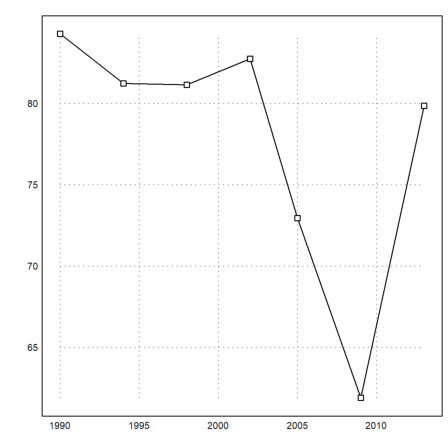
\includegraphics[keepaspectratio]{images/EMT4Statistika - Naila Khalidatus Salwa-019.png}}
\caption{images/EMT4Statistika\%20-\%20Naila\%20Khalidatus\%20Salwa-019.png}
\end{figure}

Tentukan beberapa warna untuk masing-masing pihak.

\textgreater CP:={[}rgb(0.5,0.5,0.5),red,yellow,green,rgb(0.8,0,0){]};

Sekarang kita dapat memplot hasil pemilu 2009 dan perubahannya ke dalam satu plot menggunakan gambar. Kita dapat menambahkan vektor kolom pada setiap plot.

\textgreater figure(2,1); \ldots{}\\
\textgreater{} figure(1); columnsplot(BW{[}6,3:7{]},P,color=CP); \ldots{}\\
\textgreater{} figure(2); columnsplot(BW{[}6,3:7{]}-BW{[}5,3:7{]},P,color=CP); \ldots{}\\
\textgreater{} figure(0):

\begin{figure}
\centering
\pandocbounded{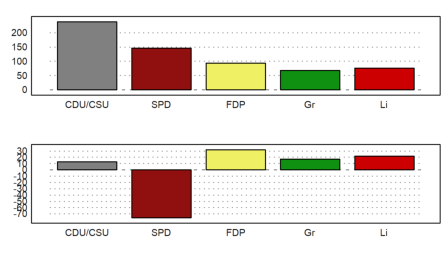
\includegraphics[keepaspectratio]{images/EMT4Statistika - Naila Khalidatus Salwa-020.png}}
\caption{images/EMT4Statistika\%20-\%20Naila\%20Khalidatus\%20Salwa-020.png}
\end{figure}

Plot data menggabungkan baris data statistik dalam satu plot.

\textgreater J:=BW{[},1{]}`; DP:=BW{[},3:7{]}'; \ldots{}\\
\textgreater{} dataplot(YT,BT',color=CP); \ldots{}\\
\textgreater{} labelbox(P,colors=CP,styles=``{[}{]}'',\textgreater points,w=0.2,x=0.3,y=0.4):

\begin{figure}
\centering
\pandocbounded{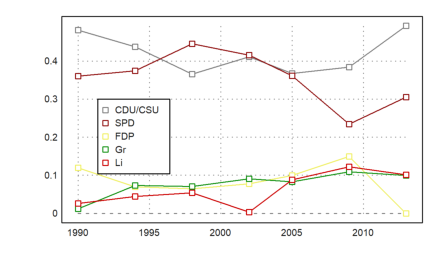
\includegraphics[keepaspectratio]{images/EMT4Statistika - Naila Khalidatus Salwa-021.png}}
\caption{images/EMT4Statistika\%20-\%20Naila\%20Khalidatus\%20Salwa-021.png}
\end{figure}

Plot kolom 3D menunjukkan deretan data statistik dalam bentuk kolom. Kami menyediakan label untuk baris dan kolom. angle adalah sudut pandang.

\textgreater columnsplot3d(BT,scols=P,srows=YT, \ldots{}\\
\textgreater{} angle=30°,ccols=CP):

\begin{figure}
\centering
\pandocbounded{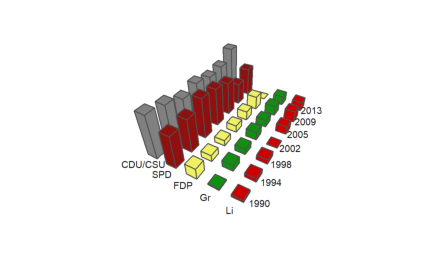
\includegraphics[keepaspectratio]{images/EMT4Statistika - Naila Khalidatus Salwa-022.png}}
\caption{images/EMT4Statistika\%20-\%20Naila\%20Khalidatus\%20Salwa-022.png}
\end{figure}

Representasi lainnya adalah plot mosaik. Perhatikan bahwa kolom-kolom pada plot mewakili kolom-kolom matriks di sini. Karena panjangnya label CDU/CSU, kita mengambil jendela yang lebih kecil dari biasanya.

\textgreater shrinkwindow(\textgreater smaller); \ldots{}\\
\textgreater{} mosaicplot(BT',srows=YT,scols=P,color=CP,style=``\#''); \ldots{}\\
\textgreater{} shrinkwindow():

\begin{figure}
\centering
\pandocbounded{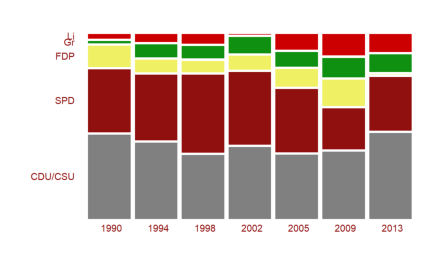
\includegraphics[keepaspectratio]{images/EMT4Statistika - Naila Khalidatus Salwa-023.png}}
\caption{images/EMT4Statistika\%20-\%20Naila\%20Khalidatus\%20Salwa-023.png}
\end{figure}

Kita juga bisa membuat diagram lingkaran. Karena warna hitam dan kuning membentuk sebuah koalisi, kita menyusun ulang elemen-elemennya.

\textgreater i={[}1,3,5,4,2{]}; piechart(BW{[}6,3:7{]}{[}i{]},color=CP{[}i{]},lab=P{[}i{]}):

\begin{figure}
\centering
\pandocbounded{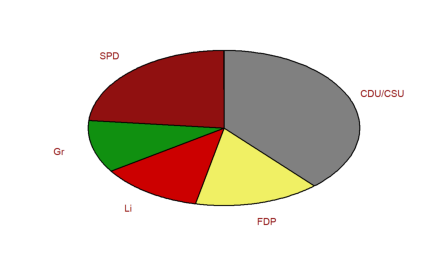
\includegraphics[keepaspectratio]{images/EMT4Statistika - Naila Khalidatus Salwa-024.png}}
\caption{images/EMT4Statistika\%20-\%20Naila\%20Khalidatus\%20Salwa-024.png}
\end{figure}

Berikut ini jenis plot yang lain.

\textgreater starplot(normal(1,10)+4,lab=1:10,\textgreater rays):

\begin{figure}
\centering
\pandocbounded{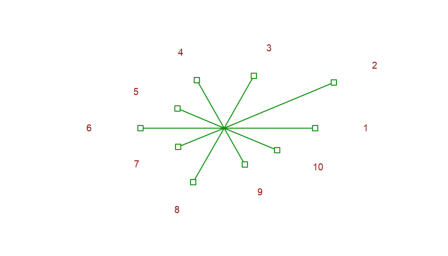
\includegraphics[keepaspectratio]{images/EMT4Statistika - Naila Khalidatus Salwa-025.png}}
\caption{images/EMT4Statistika\%20-\%20Naila\%20Khalidatus\%20Salwa-025.png}
\end{figure}

Beberapa plot di plot2d bagus untuk statika. Berikut ini adalah plot impuls dari data acak, yang terdistribusi secara seragam dalam {[}0,1{]}.

\textgreater plot2d(makeimpulse(1:10,random(1,10)),\textgreater bar):

\begin{figure}
\centering
\pandocbounded{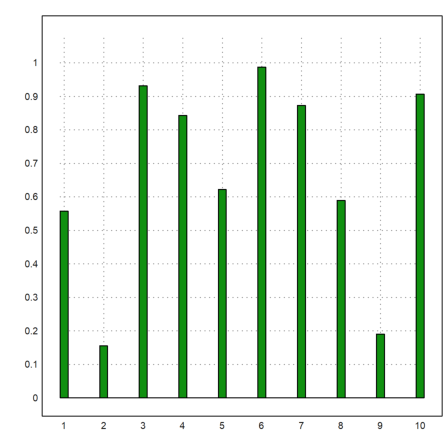
\includegraphics[keepaspectratio]{images/EMT4Statistika - Naila Khalidatus Salwa-026.png}}
\caption{images/EMT4Statistika\%20-\%20Naila\%20Khalidatus\%20Salwa-026.png}
\end{figure}

Tetapi untuk data yang terdistribusi secara eksponensial, kita mungkin memerlukan plot logaritmik.

\textgreater logimpulseplot(1:10,-log(random(1,10))*10):

\begin{figure}
\centering
\pandocbounded{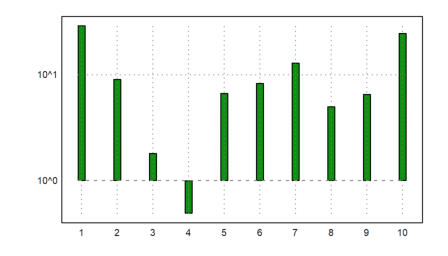
\includegraphics[keepaspectratio]{images/EMT4Statistika - Naila Khalidatus Salwa-027.png}}
\caption{images/EMT4Statistika\%20-\%20Naila\%20Khalidatus\%20Salwa-027.png}
\end{figure}

Fungsi columnsplot() lebih mudah digunakan, karena hanya membutuhkan sebuah vektor nilai. Selain itu, fungsi ini dapat mengatur labelnya menjadi apa pun yang kita inginkan, kita telah mendemonstrasikan hal ini dalam tutorial ini.

Berikut ini adalah aplikasi lain, di mana kita menghitung karakter dalam sebuah kalimat dan memplot statistik.

\textgreater v=strtochar(``the quick brown fox jumps over the lazy dog''); \ldots{}\\
\textgreater{} w=ascii(``a''):ascii(``z''); x=getmultiplicities(w,v); \ldots{}\\
\textgreater{} cw={[}{]}; for k=w; cw=cw\textbar char(k); end; \ldots{}\\
\textgreater{} columnsplot(x,lab=cw,width=0.05):

\begin{figure}
\centering
\pandocbounded{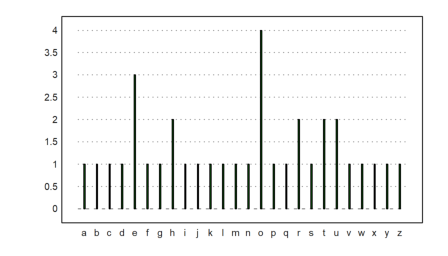
\includegraphics[keepaspectratio]{images/EMT4Statistika - Naila Khalidatus Salwa-028.png}}
\caption{images/EMT4Statistika\%20-\%20Naila\%20Khalidatus\%20Salwa-028.png}
\end{figure}

Kita juga dapat menetapkan sumbu secara manual.

\textgreater n=10; p=0.4; i=0:n; x=bin(n,i)*p\textsuperscript{i*(1-p)}(n-i); \ldots{}\\
\textgreater{} columnsplot(x,lab=i,width=0.05,\textless frame,\textless grid); \ldots{}\\
\textgreater{} yaxis(0,0:0.1:1,style=``-\textgreater{}'',\textgreater left); xaxis(0,style=``.''); \ldots{}\\
\textgreater{} label(``p'',0,0.25), label(``i'',11,0); \ldots{}\\
\textgreater{} textbox({[}``Binomial distribution'',``with p=0.4''{]}):

\begin{figure}
\centering
\pandocbounded{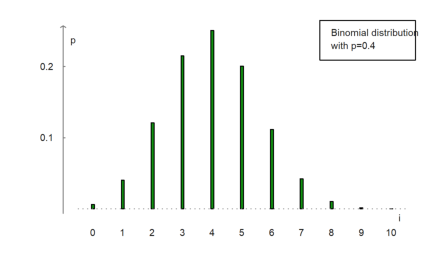
\includegraphics[keepaspectratio]{images/EMT4Statistika - Naila Khalidatus Salwa-029.png}}
\caption{images/EMT4Statistika\%20-\%20Naila\%20Khalidatus\%20Salwa-029.png}
\end{figure}

Berikut ini adalah cara untuk memplot frekuensi angka dalam vektor.

Buat vektor angka acak bilangan bulat 1 hingga 6.

\textgreater v:=intrandom(1,10,10)

\begin{verbatim}
[9,  4,  1,  3,  6,  3,  7,  9,  4,  6]
\end{verbatim}

Kemudian ekstrak nomor unik dalam v.

\textgreater vu:=unique(v)

\begin{verbatim}
[1,  3,  4,  6,  7,  9]
\end{verbatim}

Dan memplot frekuensi dalam plot kolom.

\textgreater columnsplot(getmultiplicities(vu,v),lab=vu,style=``/''):

\begin{figure}
\centering
\pandocbounded{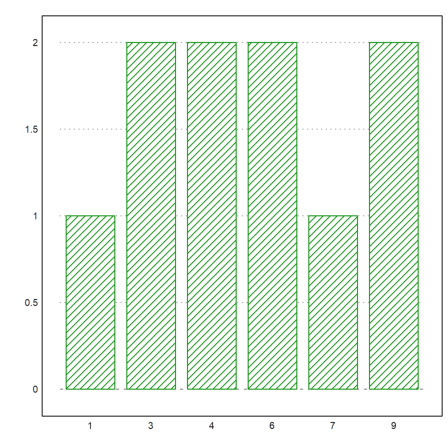
\includegraphics[keepaspectratio]{images/EMT4Statistika - Naila Khalidatus Salwa-030.png}}
\caption{images/EMT4Statistika\%20-\%20Naila\%20Khalidatus\%20Salwa-030.png}
\end{figure}

Kita ingin mendemonstrasikan fungsi untuk distribusi nilai empiris.

\textgreater x=normal(1,20);

Fungsi empdist(x,vs) membutuhkan larik nilai yang diurutkan. Jadi kita harus mengurutkan x sebelum dapat menggunakannya.

\textgreater xs=sort(x);

Kemudian kami memplot distribusi empiris dan beberapa batang kepadatan ke dalam satu plot. Alih-alih plot batang untuk distribusi, kali ini kami menggunakan plot gigi gergaji.

\textgreater figure(2,1); \ldots{}\\
\textgreater{} figure(1); plot2d(``empdist'',-4,4;xs); \ldots{}\\
\textgreater{} figure(2); plot2d(histo(x,v=-4:0.2:4,\textless bar)); \ldots{}\\
\textgreater{} figure(0):

\begin{figure}
\centering
\pandocbounded{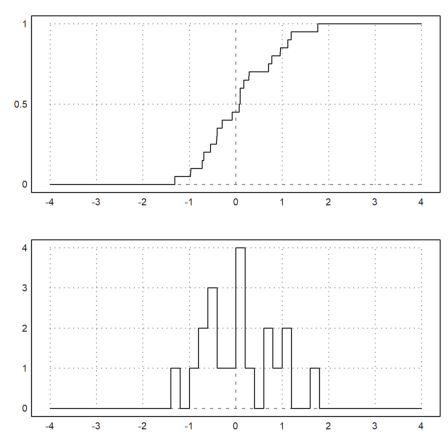
\includegraphics[keepaspectratio]{images/EMT4Statistika - Naila Khalidatus Salwa-031.png}}
\caption{images/EMT4Statistika\%20-\%20Naila\%20Khalidatus\%20Salwa-031.png}
\end{figure}

Plot sebaran mudah dilakukan di Euler dengan plot titik biasa. Grafik berikut ini menunjukkan bahwa X dan X+Y berkorelasi positif secara jelas.

\textgreater x=normal(1,100); plot2d(x,x+rotright(x),\textgreater points,style=``..''):

\begin{figure}
\centering
\pandocbounded{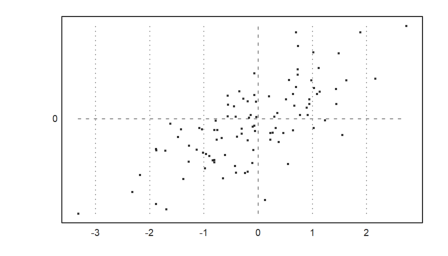
\includegraphics[keepaspectratio]{images/EMT4Statistika - Naila Khalidatus Salwa-032.png}}
\caption{images/EMT4Statistika\%20-\%20Naila\%20Khalidatus\%20Salwa-032.png}
\end{figure}

Sering kali, kita ingin membandingkan dua sampel dari distribusi yang berbeda. Hal ini dapat dilakukan dengan plot kuantil-kuantil.

Untuk pengujian, kami mencoba distribusi student-t dan distribusi eksponensial.

\textgreater x=randt(1,1000,5); y=randnormal(1,1000,mean(x),dev(x)); \ldots{}\\
\textgreater{} plot2d(``x'',r=6,style=``--'',yl=``normal'',xl=``student-t'',\textgreater vertical); \ldots{}\\
\textgreater{} plot2d(sort(x),sort(y),\textgreater points,color=red,style=``x'',\textgreater add):

\begin{figure}
\centering
\pandocbounded{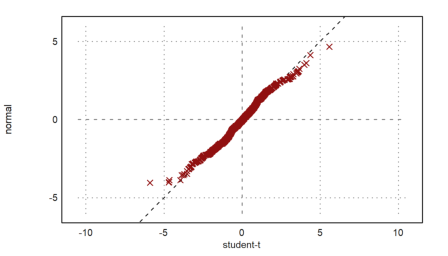
\includegraphics[keepaspectratio]{images/EMT4Statistika - Naila Khalidatus Salwa-033.png}}
\caption{images/EMT4Statistika\%20-\%20Naila\%20Khalidatus\%20Salwa-033.png}
\end{figure}

Plot tersebut dengan jelas menunjukkan bahwa nilai yang terdistribusi normal cenderung lebih kecil pada ujung yang ekstrim.

Jika kita memiliki dua distribusi dengan ukuran yang berbeda, kita dapat memperluas distribusi yang lebih kecil atau memperkecil distribusi yang lebih besar. Fungsi berikut ini bagus untuk keduanya. Fungsi ini mengambil nilai median dengan persentase antara 0 dan 1.

\textgreater function medianexpand (x,n) := median(x,p=linspace(0,1,n-1));

Mari kita bandingkan dua distribusi yang sama.

\textgreater x=random(1000); y=random(400); \ldots{}\\
\textgreater{} plot2d(``x'',0,1,style=``--''); \ldots{}\\
\textgreater{} plot2d(sort(medianexpand(x,400)),sort(y),\textgreater points,color=red,style=``x'',\textgreater add):

\begin{figure}
\centering
\pandocbounded{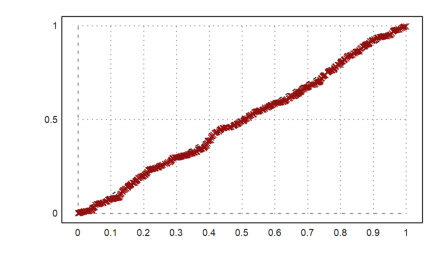
\includegraphics[keepaspectratio]{images/EMT4Statistika - Naila Khalidatus Salwa-034.png}}
\caption{images/EMT4Statistika\%20-\%20Naila\%20Khalidatus\%20Salwa-034.png}
\end{figure}

\chapter{Regresi dan Korelasi}\label{regresi-dan-korelasi}

Regresi linier dapat dilakukan dengan fungsi polyfit() atau berbagai fungsi fit.

Sebagai permulaan, kita mencari garis regresi untuk data univariat dengan polyfit(x,y,1).

\textgreater x=1:10; y={[}2,3,1,5,6,3,7,8,9,8{]}; writetable(x'\textbar y',labc={[}``x'',``y''{]})

\begin{verbatim}
         x         y
         1         2
         2         3
         3         1
         4         5
         5         6
         6         3
         7         7
         8         8
         9         9
        10         8
\end{verbatim}

Kami ingin membandingkan kecocokan tanpa bobot dan dengan bobot. Pertama, koefisien dari kecocokan linier.

\textgreater p=polyfit(x,y,1)

\begin{verbatim}
[0.733333,  0.812121]
\end{verbatim}

Sekarang, koefisien dengan bobot yang menekankan nilai terakhir.

\textgreater w \&= ``exp(-(x-10)\^{}2/10)''; pw=polyfit(x,y,1,w=w(x))

\begin{verbatim}
[4.71566,  0.38319]
\end{verbatim}

Kami menempatkan semuanya ke dalam satu plot untuk titik-titik dan garis regresi, dan untuk bobot yang digunakan.

\textgreater figure(2,1); \ldots{}\\
\textgreater{} figure(1); statplot(x,y,``b'',xl=``Regression''); \ldots{}\\
\textgreater{} plot2d(``evalpoly(x,p)'',\textgreater add,color=blue,style=``--''); \ldots{}\\
\textgreater{} plot2d(``evalpoly(x,pw)'',5,10,\textgreater add,color=red,style=``--''); \ldots{}\\
\textgreater{} figure(2); plot2d(w,1,10,\textgreater filled,style=``/'',fillcolor=red,xl=w); \ldots{}\\
\textgreater{} figure(0):

\begin{figure}
\centering
\pandocbounded{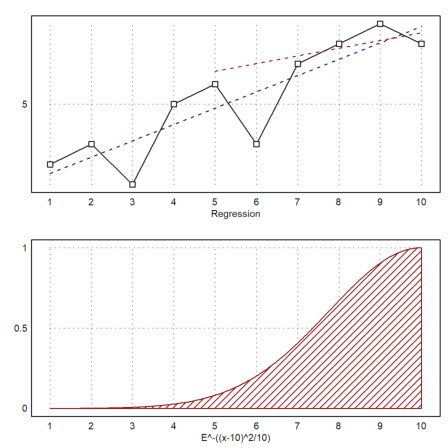
\includegraphics[keepaspectratio]{images/EMT4Statistika - Naila Khalidatus Salwa-035.png}}
\caption{images/EMT4Statistika\%20-\%20Naila\%20Khalidatus\%20Salwa-035.png}
\end{figure}

Untuk contoh lain, kita membaca survei tentang siswa, usia mereka, usia orang tua mereka, dan jumlah saudara kandung dari sebuah file.

Tabel ini berisi ``m'' dan ``f'' di kolom kedua. Kita menggunakan variabel tok2 untuk mengatur terjemahan yang tepat dan bukannya membiarkan readtable() mengumpulkan terjemahan.

\textgreater\{MS,hd\}:=readtable(``table1.dat'',tok2:={[}``m'',``f''{]}); \ldots{}\\
\textgreater{} writetable(MS,labc=hd,tok2:={[}``m'',``f''{]});

\begin{verbatim}
    Person       Sex       Age    Mother    Father  Siblings
         1         m        29        58        61         1
         2         f        26        53        54         2
         3         m        24        49        55         1
         4         f        25        56        63         3
         5         f        25        49        53         0
         6         f        23        55        55         2
         7         m        23        48        54         2
         8         m        27        56        58         1
         9         m        25        57        59         1
        10         m        24        50        54         1
        11         f        26        61        65         1
        12         m        24        50        52         1
        13         m        29        54        56         1
        14         m        28        48        51         2
        15         f        23        52        52         1
        16         m        24        45        57         1
        17         f        24        59        63         0
        18         f        23        52        55         1
        19         m        24        54        61         2
        20         f        23        54        55         1
\end{verbatim}

Bagaimana usia saling bergantung satu sama lain? Kesan pertama datang dari scatterplot berpasangan.

\textgreater scatterplots(tablecol(MS,3:5),hd{[}3:5{]}):

\begin{figure}
\centering
\pandocbounded{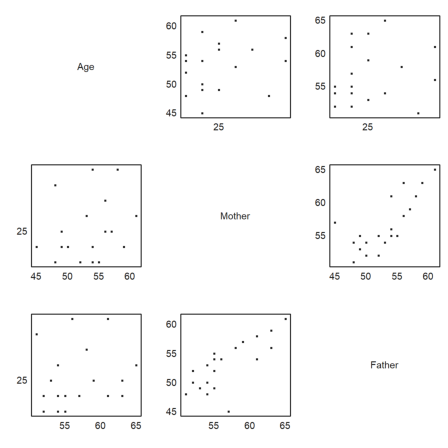
\includegraphics[keepaspectratio]{images/EMT4Statistika - Naila Khalidatus Salwa-036.png}}
\caption{images/EMT4Statistika\%20-\%20Naila\%20Khalidatus\%20Salwa-036.png}
\end{figure}

Jelas bahwa usia ayah dan ibu saling bergantung satu sama lain. Mari kita tentukan dan plot garis regresinya.

\textgreater cs:=MS{[},4:5{]}'; ps:=polyfit(cs{[}1{]},cs{[}2{]},1)

\begin{verbatim}
[17.3789,  0.740964]
\end{verbatim}

Ini jelas merupakan model yang salah. Garis regresinya adalah s = 17 + 0,74t, di mana t adalah usia ibu dan s adalah usia ayah. Perbedaan usia mungkin sedikit bergantung pada usia, tetapi tidak terlalu banyak.

Sebaliknya, kita menduga fungsi seperti s = a + t. Maka a adalah rata-rata dari s-t. Ini adalah perbedaan usia rata-rata antara ayah dan ibu.

\textgreater da:=mean(cs{[}2{]}-cs{[}1{]})

\begin{verbatim}
3.65
\end{verbatim}

Mari kita plotkan ini ke dalam satu scatter plot.

\textgreater plot2d(cs{[}1{]},cs{[}2{]},\textgreater points); \ldots{}\\
\textgreater{} plot2d(``evalpoly(x,ps)'',color=red,style=``.'',\textgreater add); \ldots{}\\
\textgreater{} plot2d(``x+da'',color=blue,\textgreater add):

\begin{figure}
\centering
\pandocbounded{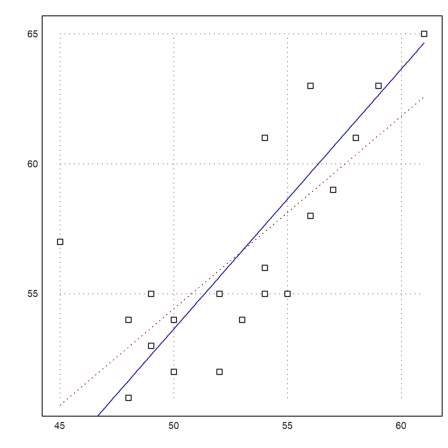
\includegraphics[keepaspectratio]{images/EMT4Statistika - Naila Khalidatus Salwa-037.png}}
\caption{images/EMT4Statistika\%20-\%20Naila\%20Khalidatus\%20Salwa-037.png}
\end{figure}

Berikut ini adalah plot kotak dari kedua usia tersebut. Ini hanya menunjukkan, bahwa usia keduanya berbeda.

\textgreater boxplot(cs,{[}``mothers'',``fathers''{]}):

\begin{figure}
\centering
\pandocbounded{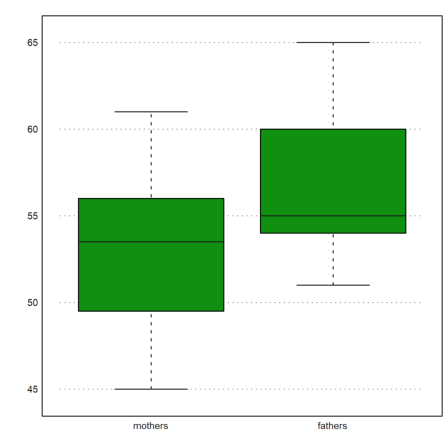
\includegraphics[keepaspectratio]{images/EMT4Statistika - Naila Khalidatus Salwa-038.png}}
\caption{images/EMT4Statistika\%20-\%20Naila\%20Khalidatus\%20Salwa-038.png}
\end{figure}

Sangat menarik bahwa perbedaan dalam median tidak sebesar perbedaan dalam mean.

\textgreater median(cs{[}2{]})-median(cs{[}1{]})

\begin{verbatim}
1.5
\end{verbatim}

Koefisien korelasi menunjukkan korelasi positif.

\textgreater correl(cs{[}1{]},cs{[}2{]})

\begin{verbatim}
0.7588307236
\end{verbatim}

Korelasi peringkat adalah ukuran untuk urutan yang sama dalam kedua vektor. Korelasi ini juga cukup positif.

\textgreater rankcorrel(cs{[}1{]},cs{[}2{]})

\begin{verbatim}
0.758925292358
\end{verbatim}

\chapter{Membuat Fungsi Baru}\label{membuat-fungsi-baru}

Tentu saja, bahasa EMT dapat digunakan untuk memprogram fungsi baru. Misalnya, kita mendefinisikan fungsi kemiringan.

\[\text{sk}(x) = \dfrac{\sqrt{n} \sum_i (x_i-m)^3}{\left(\sum_i (x_i-m)^2\right)^{3/2}}\]di mana m adalah rata-rata dari x.

\textgreater function skew (x:vector) \ldots{}

\begin{verbatim}
m=mean(x);
return sqrt(cols(x))*sum((x-m)^3)/(sum((x-m)^2))^(3/2);
endfunction
\end{verbatim}

Seperti yang Anda lihat, kita dapat dengan mudah menggunakan bahasa matriks untuk mendapatkan implementasi yang sangat singkat dan efisien. Mari kita coba fungsi ini.

\textgreater data=normal(20); skew(normal(10))

\begin{verbatim}
0.15962
\end{verbatim}

Berikut ini adalah fungsi lain, yang disebut koefisien kemencengan Pearson.

\textgreater function skew1 (x) := 3*(mean(x)-median(x))/dev(x)

\textgreater skew1(data)

\begin{verbatim}
-0.21637
\end{verbatim}

\chapter{Simulasi Monte Carlo}\label{simulasi-monte-carlo}

Euler dapat digunakan untuk mensimulasikan kejadian acak. Kita telah melihat contoh sederhana di atas. Berikut ini adalah contoh lainnya, yang mensimulasikan 1000 kali pelemparan 3 dadu, dan menanyakan distribusi dari jumlah tersebut.

\textgreater ds:=sum(intrandom(1000,3,6))'; fs=getmultiplicities(3:18,ds)

\begin{verbatim}
[6,  11,  21,  44,  73,  102,  113,  119,  134,  116,  93,  61,  55,
28,  21,  3]
\end{verbatim}

Kita bisa merencanakan ini sekarang.

\textgreater columnsplot(fs,lab=3:18):

\begin{figure}
\centering
\pandocbounded{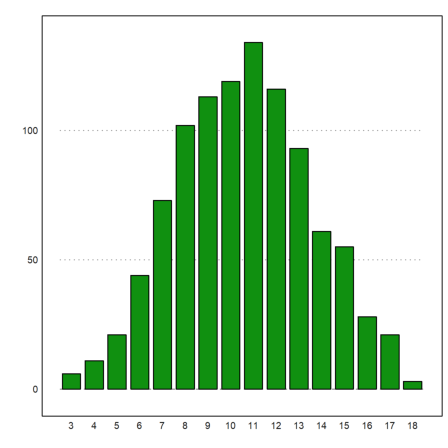
\includegraphics[keepaspectratio]{images/EMT4Statistika - Naila Khalidatus Salwa-040.png}}
\caption{images/EMT4Statistika\%20-\%20Naila\%20Khalidatus\%20Salwa-040.png}
\end{figure}

Untuk menentukan distribusi yang diharapkan tidaklah mudah. Kami menggunakan rekursi tingkat lanjut untuk hal ini.

Fungsi berikut ini menghitung jumlah cara angka k dapat direpresentasikan sebagai jumlah n angka dalam rentang 1 hingga m. Fungsi ini bekerja secara rekursif dengan cara yang jelas.

\textgreater function map countways (k; n, m) \ldots{}

\begin{verbatim}
  if n==1 then return k>=1 && k<=m
  else
    sum=0; 
    loop 1 to m; sum=sum+countways(k-#,n-1,m); end;
    return sum;
  end;
endfunction
\end{verbatim}

Berikut ini adalah hasil dari tiga lemparan dadu.

\textgreater countways(5:25,5,5)

\begin{verbatim}
[1,  5,  15,  35,  70,  121,  185,  255,  320,  365,  381,  365,  320,
255,  185,  121,  70,  35,  15,  5,  1]
\end{verbatim}

\textgreater cw=countways(3:18,3,6)

\begin{verbatim}
[1,  3,  6,  10,  15,  21,  25,  27,  27,  25,  21,  15,  10,  6,  3,
1]
\end{verbatim}

Kita akan menambahkan nilai yang diharapkan ke plot.

\textgreater plot2d(cw/6\^{}3*1000,\textgreater add); plot2d(cw/6\^{}3*1000,\textgreater points,\textgreater add):

\begin{figure}
\centering
\pandocbounded{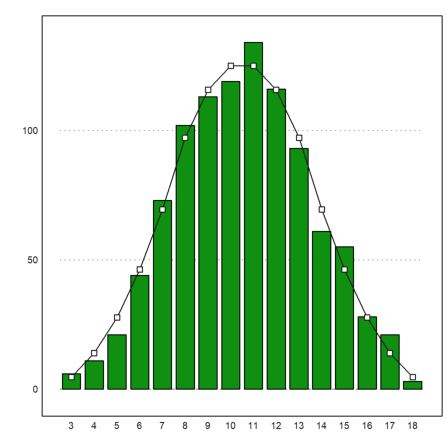
\includegraphics[keepaspectratio]{images/EMT4Statistika - Naila Khalidatus Salwa-041.png}}
\caption{images/EMT4Statistika\%20-\%20Naila\%20Khalidatus\%20Salwa-041.png}
\end{figure}

Untuk simulasi lainnya, deviasi nilai rata-rata dari n variabel acak berdistribusi normal 0-1 adalah 1/sqrt(n).

\textgreater longformat; 1/sqrt(10)

\begin{verbatim}
0.316227766017
\end{verbatim}

Mari kita periksa hal ini dengan sebuah simulasi. Kami menghasilkan 10.000 kali 10 vektor acak.

\textgreater M=normal(10000,10); dev(mean(M)')

\begin{verbatim}
0.314728610056
\end{verbatim}

\textgreater plot2d(mean(M)',\textgreater distribution):

\begin{figure}
\centering
\pandocbounded{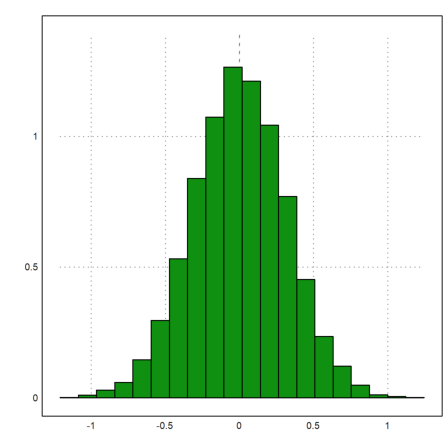
\includegraphics[keepaspectratio]{images/EMT4Statistika - Naila Khalidatus Salwa-042.png}}
\caption{images/EMT4Statistika\%20-\%20Naila\%20Khalidatus\%20Salwa-042.png}
\end{figure}

Median dari 10 bilangan acak berdistribusi normal 0-1 memiliki deviasi yang lebih besar.

\textgreater dev(median(M)')

\begin{verbatim}
0.368386999999
\end{verbatim}

Karena kita dapat dengan mudah menghasilkan jalan acak, kita dapat mensimulasikan proses Wiener. Kami mengambil 1000 langkah dari 1000 proses. Kami kemudian memplot deviasi standar dan rata-rata dari langkah ke-n dari proses-proses ini bersama dengan nilai yang diharapkan dalam warna merah.

\textgreater n=1000; m=1000; M=cumsum(normal(n,m)/sqrt(m)); \ldots{}\\
\textgreater{} t=(1:n)/n; figure(2,1); \ldots{}\\
\textgreater{} figure(1); plot2d(t,mean(M')`); plot2d(t,0,color=red,\textgreater add); \ldots{}\\
\textgreater{} figure(2); plot2d(t,dev(M')'); plot2d(t,sqrt(t),color=red,\textgreater add); \ldots{}\\
\textgreater{} figure(0):

\begin{figure}
\centering
\pandocbounded{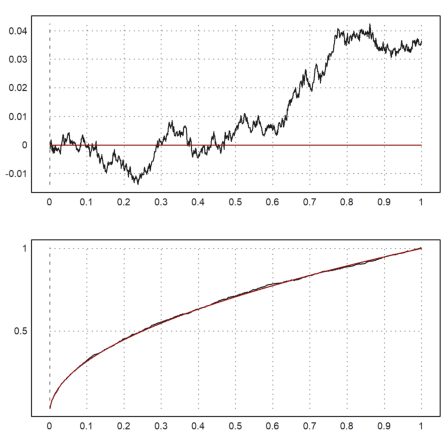
\includegraphics[keepaspectratio]{images/EMT4Statistika - Naila Khalidatus Salwa-043.png}}
\caption{images/EMT4Statistika\%20-\%20Naila\%20Khalidatus\%20Salwa-043.png}
\end{figure}

\chapter{Uji Chi-kuadrat}\label{uji-chi-kuadrat}

Uji chi-kuadrat adalah alat yang penting dalam statistik. Dalam Euler, banyak tes yang diterapkan. Semua tes ini mengembalikan kesalahan yang kita terima jika kita menolak hipotesis nol.

Sebagai contoh, kita menguji lemparan dadu untuk distribusi yang seragam. Pada 600 lemparan, kita mendapatkan nilai berikut, yang kita masukkan ke dalam uji chi-kuadrat.

\textgreater chitest({[}90,103,114,101,103,89{]},dup(100,6)')

\begin{verbatim}
0.49883
\end{verbatim}

Uji chi-square juga memiliki mode, yang menggunakan simulasi Monte Carlo untuk menguji statistik. Hasilnya seharusnya hampir sama. Parameter \textgreater p menginterpretasikan vektor y sebagai vektor probabilitas.

\textgreater chitest({[}90,103,114,101,103,89{]},dup(1/6,6)',\textgreater p,\textgreater montecarlo)

\begin{verbatim}
0.496
\end{verbatim}

Kesalahan ini terlalu besar. Jadi kita tidak bisa menolak distribusi seragam. Ini tidak membuktikan bahwa dadu kita adil. Namun kita tidak bisa menolak hipotesis kita.

Selanjutnya kita buat 1000 lemparan dadu dengan menggunakan generator bilangan acak, dan lakukan pengujian yang sama.

\textgreater n=1000; t=random({[}1,n*6{]}); chitest(count(t*6,6),dup(n,6)')

\begin{verbatim}
0.444844825624
\end{verbatim}

Mari kita uji nilai rata-rata 100 dengan uji-t.

\textgreater s=200+normal({[}1,100{]})*10; \ldots{}\\
\textgreater{} ttest(mean(s),dev(s),100,200)

\begin{verbatim}
0.20961744228
\end{verbatim}

Fungsi ttest() membutuhkan nilai rata-rata, deviasi, jumlah data, dan nilai rata-rata untuk diuji.

Sekarang mari kita periksa dua pengukuran untuk mean yang sama. Kita tolak hipotesis bahwa kedua pengukuran tersebut memiliki nilai rata-rata yang sama, jika hasilnya \textless{} 0,05.

\textgreater tcomparedata(normal(1,10),normal(1,10))

\begin{verbatim}
0.319021627346
\end{verbatim}

Jika kita menambahkan bias pada satu distribusi, kita akan mendapatkan lebih banyak penolakan. Ulangi simulasi ini beberapa kali untuk melihat efeknya.

\textgreater tcomparedata(normal(1,10),normal(1,10)+2)

\begin{verbatim}
5.6993803492e-05
\end{verbatim}

Pada contoh berikut, kami menghasilkan 20 lemparan dadu acak sebanyak 100 kali dan menghitung jumlah dadu yang muncul. Rata-rata harus ada 20/6 = 3,3 mata dadu.

\textgreater R=random(100,20); R=sum(R*6\textless=1)'; mean(R)

\begin{verbatim}
3.65
\end{verbatim}

Sekarang kita bandingkan jumlah tersebut dengan distribusi binomial. Pertama, kita memplot distribusi angka satu.

\textgreater plot2d(R,distribution=max(R)+1,even=1,style=``\textbackslash/''):

\begin{figure}
\centering
\pandocbounded{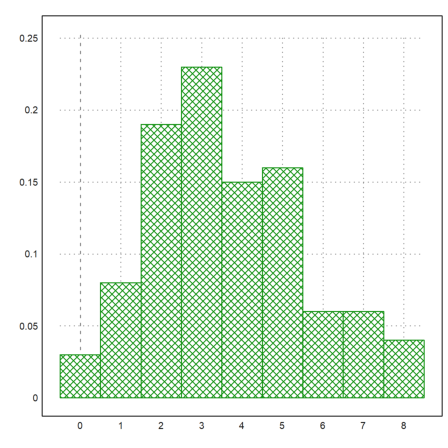
\includegraphics[keepaspectratio]{images/EMT4Statistika - Naila Khalidatus Salwa-044.png}}
\caption{images/EMT4Statistika\%20-\%20Naila\%20Khalidatus\%20Salwa-044.png}
\end{figure}

\textgreater t=count(R,21);

Kemudian kami menghitung nilai yang diharapkan.

\textgreater n=0:20; b=bin(20,n)*(1/6)\textsuperscript{n*(5/6)}(20-n)*100;

Kami harus mengumpulkan beberapa angka untuk mendapatkan kategori yang cukup besar.

\textgreater t1=sum(t{[}1:2{]})\textbar t{[}3:7{]}\textbar sum(t{[}8:21{]}); \ldots{}\\
\textgreater{} b1=sum(b{[}1:2{]})\textbar b{[}3:7{]}\textbar sum(b{[}8:21{]});

Uji chi-square menolak hipotesis bahwa distribusi kita adalah distribusi binomial, jika hasilnya \textless0,05.

\textgreater chitest(t1,b1)

\begin{verbatim}
0.0410596511653
\end{verbatim}

Contoh berikut ini berisi hasil dari dua kelompok orang (katakanlah laki-laki dan perempuan) yang memberikan suara untuk satu dari enam partai.

\textgreater A={[}23,37,43,52,64,74;27,39,41,49,63,76{]}; \ldots{}\\
\textgreater{} writetable(A,wc=6,labr={[}``m'',``f''{]},labc=1:6)

\begin{verbatim}
           1     2     3     4     5     6
     m    23    37    43    52    64    74
     f    27    39    41    49    63    76
\end{verbatim}

Kami ingin menguji independensi suara dari jenis kelamin. Uji tabel chi\^{}2 melakukan hal ini. Hasilnya terlalu besar untuk menolak independensi. Jadi kita tidak dapat mengatakan, jika pemungutan suara tergantung pada jenis kelamin dari data ini.

\textgreater tabletest(A)

\begin{verbatim}
0.990701632326
\end{verbatim}

Berikut ini adalah tabel yang diharapkan, jika kita mengasumsikan frekuensi pemungutan suara yang diamati.

\textgreater writetable(expectedtable(A),wc=6,dc=1,labr={[}``m'',``f''{]},labc=1:6)

\begin{verbatim}
           1     2     3     4     5     6
     m  24.9  37.9  41.9  50.3  63.3  74.7
     f  25.1  38.1  42.1  50.7  63.7  75.3
\end{verbatim}

Kita dapat menghitung koefisien kontingensi terkoreksi. Karena koefisien ini sangat dekat dengan 0, kami menyimpulkan bahwa pemungutan suara tidak bergantung pada jenis kelamin.

\textgreater contingency(A)

\begin{verbatim}
0.0427225484717
\end{verbatim}

\chapter{Uji-F}\label{uji-f}

Selanjutnya kita menggunakan analisis varians (F-test) untuk menguji tiga sampel data yang terdistribusi secara normal untuk nilai rata-rata yang sama. Metode ini disebut ANOVA (analisis varians). Dalam Euler, fungsi varanalysis() digunakan.

\textgreater x1={[}109,111,98,119,91,118,109,99,115,109,94{]}; mean(x1),

\begin{verbatim}
106.55
\end{verbatim}

\textgreater x2={[}120,124,115,139,114,110,113,120,117{]}; mean(x2),

\begin{verbatim}
119.11
\end{verbatim}

\textgreater x3={[}120,112,115,110,105,134,105,130,121,111{]}; mean(x3)

\begin{verbatim}
116.3
\end{verbatim}

\textgreater varanalysis(x1,x2,x3)

\begin{verbatim}
0.0138048221371
\end{verbatim}

Ini berarti, kami menolak hipotesis nilai rata-rata yang sama. Kami melakukan ini dengan probabilitas kesalahan sebesar 1,3\%.

Ada juga uji median, yang menolak sampel data dengan distribusi rata-rata yang berbeda dengan menguji median dari sampel gabungan.

\textgreater a={[}56,66,68,49,61,53,45,58,54{]};

\textgreater b={[}72,81,51,73,69,78,59,67,65,71,68,71{]};

\textgreater mediantest(a,b)

\begin{verbatim}
0.0241724220052
\end{verbatim}

Uji lain tentang kesetaraan adalah uji peringkat. Uji ini jauh lebih tajam daripada uji median.

\textgreater ranktest(a,b)

\begin{verbatim}
0.00199969612469
\end{verbatim}

Dalam contoh berikut, kedua distribusi memiliki rata-rata yang sama.

\textgreater ranktest(random(1,100),random(1,50)*3-1)

\begin{verbatim}
0.0174730789662
\end{verbatim}

Sekarang mari kita coba mensimulasikan dua perawatan a dan b yang diterapkan pada orang yang berbeda.

\textgreater a={[}8.0,7.4,5.9,9.4,8.6,8.2,7.6,8.1,6.2,8.9{]};

\textgreater b={[}6.8,7.1,6.8,8.3,7.9,7.2,7.4,6.8,6.8,8.1{]};

Uji signum memutuskan, apakah a lebih baik daripada b.

\textgreater signtest(a,b)

\begin{verbatim}
0.0546875
\end{verbatim}

Ini adalah kesalahan yang terlalu besar. Kita tidak dapat menolak bahwa a sama baiknya dengan b.

Uji Wilcoxon lebih tajam daripada uji ini, tetapi bergantung pada nilai kuantitatif dari perbedaan.

\textgreater wilcoxon(a,b)

\begin{verbatim}
0.0296680599405
\end{verbatim}

Mari kita coba dua pengujian lagi dengan menggunakan rangkaian yang dihasilkan.

\textgreater wilcoxon(normal(1,20),normal(1,20)-1)

\begin{verbatim}
0.00359458419569
\end{verbatim}

\textgreater wilcoxon(normal(1,20),normal(1,20))

\begin{verbatim}
0.0200218990361
\end{verbatim}

\chapter{Bilangan Acak}\label{bilangan-acak}

Berikut ini adalah tes untuk generator bilangan acak. Euler menggunakan generator yang sangat bagus, jadi kita tidak perlu mengharapkan adanya masalah.

Pertama, kita akan membangkitkan sepuluh juta bilangan acak dalam {[}0,1{]}.

\textgreater n:=10000000; r:=random(1,n);

Selanjutnya, kami menghitung jarak antara dua angka yang kurang dari 0,05.

\textgreater a:=0.05; d:=differences(nonzeros(r\textless a));

Terakhir, kami memplot berapa kali, setiap jarak yang terjadi, dan membandingkannya dengan nilai yang diharapkan.

\textgreater m=getmultiplicities(1:100,d); plot2d(m); \ldots{}\\
\textgreater{} plot2d(``n*(1-a)\textsuperscript{(x-1)*a}2'',color=red,\textgreater add):

\begin{figure}
\centering
\pandocbounded{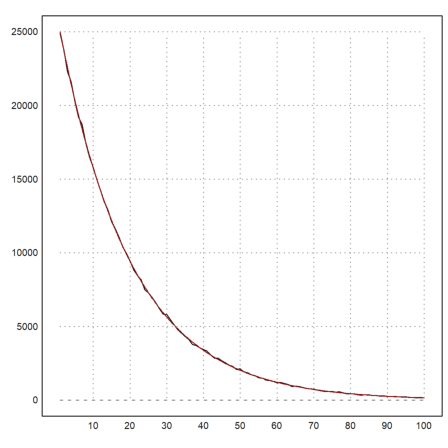
\includegraphics[keepaspectratio]{images/EMT4Statistika - Naila Khalidatus Salwa-045.png}}
\caption{images/EMT4Statistika\%20-\%20Naila\%20Khalidatus\%20Salwa-045.png}
\end{figure}

Menghapus data.

\textgreater remvalue n;

\chapter{Pengantar untuk Pengguna Proyek R}\label{pengantar-untuk-pengguna-proyek-r}

Jelas, EMT tidak bersaing dengan R sebagai paket statistik. Namun, ada banyak prosedur dan fungsi statistik yang tersedia di EMT juga. Jadi EMT dapat memenuhi kebutuhan dasar. Bagaimanapun, EMT hadir dengan paket numerik dan sistem aljabar komputer.

Notebook ini diperuntukkan bagi Anda yang sudah terbiasa dengan R, tetapi perlu mengetahui perbedaan sintaks EMT dan R. Kami mencoba memberikan gambaran umum mengenai hal-hal yang jelas dan kurang jelas yang perlu Anda ketahui.

Selain itu, kami juga membahas cara-cara untuk bertukar data di antara kedua sistem tersebut.

Perhatikan bahwa ini adalah pekerjaan yang sedang berlangsung.

\chapter{Sintaks Dasar}\label{sintaks-dasar}

Hal pertama yang Anda pelajari dalam R adalah membuat sebuah vektor. Dalam EMT, perbedaan utamanya adalah bahwa operator : dapat mengambil ukuran langkah. Selain itu, operator ini memiliki daya ikat yang rendah.

\textgreater n=10; 0:n/20:n-1

\begin{verbatim}
[0,  0.5,  1,  1.5,  2,  2.5,  3,  3.5,  4,  4.5,  5,  5.5,  6,  6.5,
7,  7.5,  8,  8.5,  9]
\end{verbatim}

Fungsi c() tidak ada. Anda dapat menggunakan vektor untuk menggabungkan beberapa hal.

Contoh berikut ini, seperti banyak contoh lainnya, berasal dari ``Introduksi ke R'' yang disertakan dengan proyek R. Jika Anda membaca PDF ini, Anda akan menemukan bahwa saya mengikuti alurnya dalam tutorial ini.

\textgreater x={[}10.4, 5.6, 3.1, 6.4, 21.7{]}; {[}x,0,x{]}

\begin{verbatim}
[10.4,  5.6,  3.1,  6.4,  21.7,  0,  10.4,  5.6,  3.1,  6.4,  21.7]
\end{verbatim}

Operator titik dua dengan ukuran langkah EMT digantikan oleh fungsi seq() dalam R. Kita dapat menulis fungsi ini dalam EMT.

\textgreater function seq(a,b,c) := a:b:c; \ldots{}\\
\textgreater{} seq(0,-0.1,-1)

\begin{verbatim}
[0,  -0.1,  -0.2,  -0.3,  -0.4,  -0.5,  -0.6,  -0.7,  -0.8,  -0.9,  -1]
\end{verbatim}

Fungsi rep() dari R tidak ada dalam EMT. Untuk input vektor, dapat dituliskan sebagai berikut.

\textgreater function rep(x:vector,n:index) := flatten(dup(x,n)); \ldots{}\\
\textgreater{} rep(x,2)

\begin{verbatim}
[10.4,  5.6,  3.1,  6.4,  21.7,  10.4,  5.6,  3.1,  6.4,  21.7]
\end{verbatim}

Perhatikan bahwa ``='' atau ``:='' digunakan untuk penugasan. Operator ``-\textgreater{}'' digunakan untuk unit dalam EMT.

\textgreater125km -\textgreater{} '' miles''

\begin{verbatim}
77.6713990297 miles
\end{verbatim}

Operator ``\textless-'' untuk penugasan juga menyesatkan, dan bukan ide yang baik untuk R. Berikut ini akan membandingkan a dan -4 dalam EMT.

\textgreater a=2; a\textless-4

\begin{verbatim}
0
\end{verbatim}

Dalam R, ``a\textless-4\textless3'' bisa digunakan, tetapi ``a\textless-4\textless-3'' tidak. Saya juga mengalami ambiguitas yang sama di EMT, tetapi saya mencoba untuk menghilangkannya.

EMT dan R memiliki vektor dengan tipe boolean. Tetapi dalam EMT, angka 0 dan 1 digunakan untuk mewakili salah dan benar. Dalam R, nilai benar dan salah tetap dapat digunakan dalam aritmatika biasa seperti dalam EMT.

\textgreater x\textless5, \%*x

\begin{verbatim}
[0,  0,  1,  0,  0]
[0,  0,  3.1,  0,  0]
\end{verbatim}

EMT melempar kesalahan atau menghasilkan NAN tergantung pada flag ``kesalahan''.

\textgreater errors off; 0/0, isNAN(sqrt(-1)), errors on;

\begin{verbatim}
NAN
1
\end{verbatim}

String sama saja dalam R dan EMT. Keduanya berada di lokal saat ini, bukan di Unicode.

Dalam R ada paket-paket untuk Unicode. Dalam EMT, sebuah string dapat berupa string Unicode. Sebuah string Unicode dapat diterjemahkan ke pengkodean lokal dan sebaliknya. Selain itu, u''\ldots'' dapat berisi entitas HTML.

\textgreater u''© Ren\&eacut; Grothmann''

\begin{verbatim}
© René Grothmann
\end{verbatim}

Berikut ini mungkin atau mungkin tidak ditampilkan dengan benar pada sistem Anda sebagai A dengan titik dan tanda hubung di atasnya. Hal ini tergantung pada jenis huruf yang Anda gunakan.

\textgreater chartoutf({[}480{]})

\begin{verbatim}
Ǡ
\end{verbatim}

Penggabungan string dilakukan dengan ``+'' atau ``\textbar{}''. Ini dapat menyertakan angka, yang akan dicetak dalam format saat ini.

\textgreater{}``pi =''+pi

\begin{verbatim}
pi = 3.14159265359
\end{verbatim}

\chapter{Pengindeksan}\label{pengindeksan}

Sebagian besar waktu, ini akan bekerja seperti pada R.

Tetapi EMT akan menginterpretasikan indeks negatif dari bagian belakang vektor, sementara R menginterpretasikan x{[}n{]} sebagai x tanpa elemen ke-n.

\textgreater x, x{[}1:3{]}, x{[}-2{]}

\begin{verbatim}
[10.4,  5.6,  3.1,  6.4,  21.7]
[10.4,  5.6,  3.1]
6.4
\end{verbatim}

Perilaku R dapat dicapai dalam EMT dengan drop().

\textgreater drop(x,2)

\begin{verbatim}
[10.4,  3.1,  6.4,  21.7]
\end{verbatim}

Vektor logika tidak diperlakukan secara berbeda dengan indeks di EMT, berbeda dengan R. Anda perlu mengekstrak elemen yang bukan nol terlebih dahulu di EMT.

\textgreater x, x\textgreater5, x{[}nonzeros(x\textgreater5){]}

\begin{verbatim}
Variable x not found!
Error in:
x, x&gt;5, x[nonzeros(x&gt;5)] ...
 ^
\end{verbatim}

Sama seperti di R, vektor indeks dapat berisi pengulangan.

\begin{verbatim}
[10.4,  5.6,  5.6,  10.4]
\end{verbatim}

Namun pemberian nama untuk indeks tidak dimungkinkan dalam EMT. Untuk paket statistik, hal ini mungkin diperlukan untuk memudahkan akses ke elemen-elemen vektor.

Untuk meniru perilaku ini, kita dapat mendefinisikan sebuah fungsi sebagai berikut.

\textgreater function sel (v,i,s) := v{[}indexof(s,i){]}; \ldots{}\\
\textgreater{} s={[}``first'',``second'',``third'',``fourth''{]}; sel(x,{[}``first'',``third''{]},s)

\begin{verbatim}
Trying to overwrite protected function sel!
Error in:
function sel (v,i,s) := v[indexof(s,i)]; ... ...
             ^
[10.4,  3.1]
\end{verbatim}

\chapter{Tipe Data}\label{tipe-data}

EMT memiliki tipe data yang lebih tetap dibandingkan R. Jelas, dalam R terdapat vektor yang berkembang. Anda bisa mengatur sebuah vektor numerik kosong v dan memberikan sebuah nilai pada elemen v{[}17{]}. Hal ini tidak mungkin dilakukan dalam EMT.

Hal berikut ini sedikit tidak efisien.

\textgreater v={[}{]}; for i=1 to 10000; v=v\textbar i; end;

EMT sekarang akan membangun vektor dengan v dan i yang ditambahkan pada tumpukan dan menyalin vektor tersebut kembali ke variabel global v.

Pendefinisian awal vektor yang lebih efisien.

\textgreater v=zeros(10000); for i=1 to 10000; v{[}i{]}=i; end;

Untuk mengubah jenis tanggal di EMT, Anda dapat menggunakan fungsi seperti complex().

\textgreater complex(1:4)

\begin{verbatim}
[ 1+0i ,  2+0i ,  3+0i ,  4+0i  ]
\end{verbatim}

Konversi ke string hanya dapat dilakukan untuk tipe data dasar. Format saat ini digunakan untuk penggabungan string sederhana. Tetapi ada fungsi-fungsi seperti print() atau frac().

Untuk vektor, Anda dapat dengan mudah menulis fungsi Anda sendiri.

\textgreater function tostr (v) \ldots{}

\begin{verbatim}
s="[";
loop 1 to length(v);
   s=s+print(v[#],2,0);
   if #<length(v) then s=s+","; endif;
end;
return s+"]";
endfunction
\end{verbatim}

\textgreater tostr(linspace(0,1,10))

\begin{verbatim}
[0.00,0.10,0.20,0.30,0.40,0.50,0.60,0.70,0.80,0.90,1.00]
\end{verbatim}

Untuk komunikasi dengan Maxima, ada fungsi convertmxm(), yang juga dapat digunakan untuk memformat vektor untuk output.

\textgreater convertmxm(1:10)

\begin{verbatim}
[1,2,3,4,5,6,7,8,9,10]
\end{verbatim}

Untuk Latex, perintah tex dapat digunakan untuk mendapatkan perintah Latex.

\textgreater tex(\&{[}1,2,3{]})

\begin{verbatim}
\left[ 1 , 2 , 3 \right] 
\end{verbatim}

\chapter{Faktor dan Tabel}\label{faktor-dan-tabel}

Dalam pengantar R ada sebuah contoh yang disebut faktor.

Berikut ini adalah daftar wilayah dari 30 negara bagian.

\textgreater austates = {[}``tas'', ``sa'', ``qld'', ``nsw'', ``nsw'', ``nt'', ``wa'', ``wa'', \ldots{}\\
\textgreater{} ``qld'', ``vic'', ``nsw'', ``vic'', ``qld'', ``qld'', ``sa'', ``tas'', \ldots{}\\
\textgreater{} ``sa'', ``nt'', ``wa'', ``vic'', ``qld'', ``nsw'', ``nsw'', ``wa'', \ldots{}\\
\textgreater{} ``sa'', ``act'', ``nsw'', ``vic'', ``vic'', ``act''{]};

Asumsikan, kita memiliki pendapatan yang sesuai di setiap negara bagian.

\textgreater incomes = {[}60, 49, 40, 61, 64, 60, 59, 54, 62, 69, 70, 42, 56, \ldots{}\\
\textgreater{} 61, 61, 61, 58, 51, 48, 65, 49, 49, 41, 48, 52, 46, \ldots{}\\
\textgreater{} 59, 46, 58, 43{]};

Sekarang, kita ingin menghitung rata-rata pendapatan di wilayah tersebut. Sebagai sebuah program statistik, R memiliki fungsi factor() dan tappy() untuk hal ini.

EMT dapat melakukan hal ini dengan mencari indeks dari wilayah-wilayah di dalam daftar unik dari wilayah-wilayah tersebut.

\textgreater auterr=sort(unique(austates)); f=indexofsorted(auterr,austates)

\begin{verbatim}
[6,  5,  4,  2,  2,  3,  8,  8,  4,  7,  2,  7,  4,  4,  5,  6,  5,  3,
8,  7,  4,  2,  2,  8,  5,  1,  2,  7,  7,  1]
\end{verbatim}

Pada titik ini, kita dapat menulis fungsi perulangan kita sendiri untuk melakukan berbagai hal untuk satu faktor saja.

Atau kita dapat meniru fungsi tapply() dengan cara berikut.

\textgreater function map tappl (i; f\$:call, cat, x) \ldots{}

\begin{verbatim}
u=sort(unique(cat));
f=indexof(u,cat);
return f$(x[nonzeros(f==indexof(u,i))]);
endfunction
\end{verbatim}

Ini sedikit tidak efisien, karena menghitung wilayah unik untuk setiap i, tetapi berfungsi.

\textgreater tappl(auterr,``mean'',austates,incomes)

\begin{verbatim}
[44.5,  57.3333333333,  55.5,  53.6,  55,  60.5,  56,  52.25]
\end{verbatim}

Perhatikan bahwa ini bekerja untuk setiap vektor wilayah.

\textgreater tappl({[}``act'',``nsw''{]},``mean'',austates,incomes)

\begin{verbatim}
[44.5,  57.3333333333]
\end{verbatim}

Sekarang, paket statistik EMT mendefinisikan tabel seperti halnya di R. Fungsi readtable() dan writetable() dapat digunakan untuk input dan output.

Jadi kita dapat mencetak rata-rata pendapatan negara di wilayah dengan cara yang ramah.

\textgreater writetable(tappl(auterr,``mean'',austates,incomes),labc=auterr,wc=7)

\begin{verbatim}
    act    nsw     nt    qld     sa    tas    vic     wa
   44.5  57.33   55.5   53.6     55   60.5     56  52.25
\end{verbatim}

Kita juga dapat mencoba meniru perilaku R sepenuhnya.

Faktor-faktor tersebut harus disimpan dengan jelas dalam sebuah koleksi dengan jenis dan kategorinya (negara bagian dan wilayah dalam contoh kita). Untuk EMT, kita menambahkan indeks yang telah dihitung sebelumnya.

\textgreater function makef (t) \ldots{}

\begin{verbatim}
## Factor data
## Returns a collection with data t, unique data, indices.
## See: tapply
u=sort(unique(t));
return {{t,u,indexofsorted(u,t)}};
endfunction
\end{verbatim}

\textgreater statef=makef(austates);

Sekarang elemen ketiga dari koleksi ini akan berisi indeks.

\textgreater statef{[}3{]}

\begin{verbatim}
[6,  5,  4,  2,  2,  3,  8,  8,  4,  7,  2,  7,  4,  4,  5,  6,  5,  3,
8,  7,  4,  2,  2,  8,  5,  1,  2,  7,  7,  1]
\end{verbatim}

Sekarang kita dapat meniru tapply() dengan cara berikut. Ini akan mengembalikan sebuah tabel sebagai kumpulan data tabel dan judul kolom.

\textgreater function tapply (t:vector,tf,f\$:call) \ldots{}

\begin{verbatim}
## Makes a table of data and factors
## tf : output of makef()
## See: makef
uf=tf[2]; f=tf[3]; x=zeros(length(uf));
for i=1 to length(uf);
   ind=nonzeros(f==i);
   if length(ind)==0 then x[i]=NAN;
   else x[i]=f$(t[ind]);
   endif;
end;
return {{x,uf}};
endfunction
\end{verbatim}

Kami tidak menambahkan banyak pemeriksaan tipe di sini. Satu-satunya tindakan pencegahan adalah kategori (faktor) yang tidak memiliki data. Tetapi kita harus memeriksa panjang t yang benar dan ketepatan koleksi tf.

Tabel ini bisa dicetak sebagai sebuah tabel dengan writetable().

\textgreater writetable(tapply(incomes,statef,``mean''),wc=7)

\begin{verbatim}
    act    nsw     nt    qld     sa    tas    vic     wa
   44.5  57.33   55.5   53.6     55   60.5     56  52.25
\end{verbatim}

\chapter{Array}\label{array}

EMT hanya memiliki dua dimensi untuk array. Tipe datanya disebut matriks. Akan lebih mudah untuk menulis fungsi untuk dimensi yang lebih tinggi atau pustaka C untuk ini.

R memiliki lebih dari dua dimensi. Dalam R, larik adalah sebuah vektor dengan sebuah bidang dimensi.

Dalam EMT, sebuah vektor adalah sebuah matriks dengan satu baris. Ini bisa dibuat menjadi sebuah matriks dengan redim().

\textgreater shortformat; X=redim(1:20,4,5)

\begin{verbatim}
        1         2         3         4         5 
        6         7         8         9        10 
       11        12        13        14        15 
       16        17        18        19        20 
\end{verbatim}

Ekstraksi baris dan kolom, atau sub-matriks, sama seperti di R.

\textgreater X{[},2:3{]}

\begin{verbatim}
        2         3 
        7         8 
       12        13 
       17        18 
\end{verbatim}

Namun, dalam R dimungkinkan untuk menetapkan daftar indeks tertentu dari vektor ke suatu nilai. Hal yang sama juga dapat dilakukan dalam EMT hanya dengan sebuah perulangan.

\textgreater function setmatrixvalue (M, i, j, v) \ldots{}

\begin{verbatim}
loop 1 to max(length(i),length(j),length(v))
   M[i{#},j{#}] = v{#};
end;
endfunction
\end{verbatim}

Kami mendemonstrasikan hal ini untuk menunjukkan bahwa matriks diteruskan dengan referensi dalam EMT. Jika Anda tidak ingin mengubah matriks asli M, Anda perlu menyalinnya dalam fungsi.

\textgreater setmatrixvalue(X,1:3,3:-1:1,0); X,

\begin{verbatim}
        1         2         0         4         5 
        6         0         8         9        10 
        0        12        13        14        15 
       16        17        18        19        20 
\end{verbatim}

Hasil kali luar dalam EMT hanya dapat dilakukan di antara vektor. Hal ini dilakukan secara otomatis karena bahasa matriks. Satu vektor harus berupa vektor kolom dan vektor baris.

\textgreater(1:5)*(1:5)'

\begin{verbatim}
        1         2         3         4         5 
        2         4         6         8        10 
        3         6         9        12        15 
        4         8        12        16        20 
        5        10        15        20        25 
\end{verbatim}

Dalam pengantar PDF untuk R ada sebuah contoh, yang menghitung distribusi ab-cd untuk a, b, c, d yang dipilih dari 0 sampai n secara acak. Solusinya dalam R adalah membentuk sebuah matriks 4 dimensi dan menjalankan table() di atasnya.

Tentu saja, ini bisa dicapai dengan sebuah perulangan. Tetapi perulangan tidak efektif dalam EMT atau R. Dalam EMT, kita bisa menulis perulangan dalam C dan itu adalah solusi tercepat.

Tetapi kita ingin meniru perilaku R. Untuk ini, kita perlu meratakan perkalian ab dan membuat sebuah matriks ab-cd.

\textgreater a=0:6; b=a'; p=flatten(a*b); q=flatten(p-p'); \ldots{}\\
\textgreater{} u=sort(unique(q)); f=getmultiplicities(u,q); \ldots{}\\
\textgreater{} statplot(u,f,``h''):

\begin{figure}
\centering
\pandocbounded{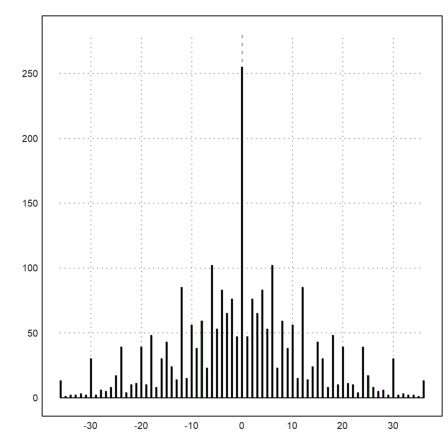
\includegraphics[keepaspectratio]{images/EMT4Statistika - Naila Khalidatus Salwa-046.png}}
\caption{images/EMT4Statistika\%20-\%20Naila\%20Khalidatus\%20Salwa-046.png}
\end{figure}

Selain kelipatan yang tepat, EMT dapat menghitung frekuensi dalam vektor.

\textgreater getfrequencies(q,-50:10:50)

\begin{verbatim}
[0,  23,  132,  316,  602,  801,  333,  141,  53,  0]
\end{verbatim}

Cara yang paling mudah untuk memplot ini sebagai distribusi adalah sebagai berikut.

\textgreater plot2d(q,distribution=11):

\begin{figure}
\centering
\pandocbounded{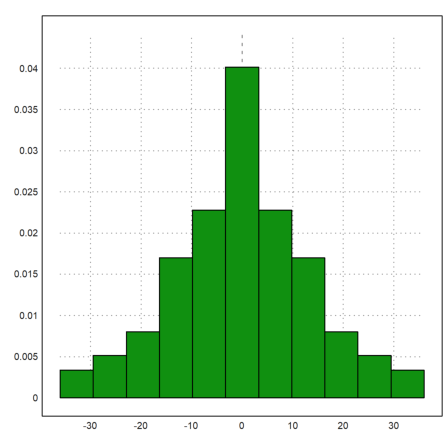
\includegraphics[keepaspectratio]{images/EMT4Statistika - Naila Khalidatus Salwa-047.png}}
\caption{images/EMT4Statistika\%20-\%20Naila\%20Khalidatus\%20Salwa-047.png}
\end{figure}

Tetapi juga memungkinkan untuk menghitung jumlah dalam interval yang dipilih sebelumnya. Tentu saja, berikut ini menggunakan getfrequencies() secara internal.

Karena fungsi histo() mengembalikan frekuensi, kita perlu menskalakannya sehingga integral di bawah grafik batang adalah 1.

\textgreater\{x,y\}=histo(q,v=-55:10:55); y=y/sum(y)/differences(x); \ldots{}\\
\textgreater{} plot2d(x,y,\textgreater bar,style=``/''):

\begin{figure}
\centering
\pandocbounded{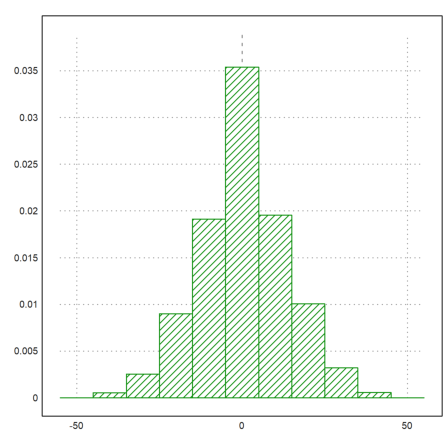
\includegraphics[keepaspectratio]{images/EMT4Statistika - Naila Khalidatus Salwa-048.png}}
\caption{images/EMT4Statistika\%20-\%20Naila\%20Khalidatus\%20Salwa-048.png}
\end{figure}

\chapter{Daftar}\label{daftar}

EMT memiliki dua jenis daftar. Yang pertama adalah daftar global yang dapat diubah, dan yang kedua adalah jenis daftar yang tidak dapat diubah. Kita tidak peduli dengan daftar global di sini.

Tipe daftar yang tidak dapat diubah disebut koleksi dalam EMT. Ia berperilaku seperti struktur dalam C, tetapi elemen-elemennya hanya diberi nomor dan tidak diberi nama.

\textgreater L=\{\{``Fred'',``Flintstone'',40,{[}1990,1992{]}\}\}

\begin{verbatim}
Fred
Flintstone
40
[1990,  1992]
\end{verbatim}

Saat ini elemen-elemen tersebut tidak memiliki nama, meskipun nama dapat ditetapkan untuk tujuan khusus. Elemen-elemen tersebut diakses dengan angka.

\textgreater(L{[}4{]}){[}2{]}

\begin{verbatim}
1992
\end{verbatim}

\chapter{Input dan Output File (Membaca dan Menulis Data)}\label{input-dan-output-file-membaca-dan-menulis-data}

Kita mungkin sering ingin mengimpor matriks data dari sumber lain ke EMT. Tutorial ini akan menjelaskan kepada Anda tentang berbagai cara untuk melakukan hal tersebut. Fungsi yang sederhana adalah writematrix() dan readmatrix().

Mari kita tunjukkan bagaimana cara membaca dan menulis sebuah vektor real ke sebuah file.

\textgreater a=random(1,100); mean(a), dev(a),

\begin{verbatim}
0.51101
0.29057
\end{verbatim}

Untuk menulis data ke sebuah berkas, kita menggunakan fungsi writematrix().

Karena pengenalan ini kemungkinan besar berada dalam sebuah direktori, di mana pengguna tidak memiliki akses tulis, kita menulis data ke direktori home pengguna. Untuk notebook sendiri, hal ini tidak diperlukan, karena file data akan ditulis ke dalam direktori yang sama.

\textgreater filename=``test.dat'';

Sekarang kita menulis vektor kolom a' ke file. Hal ini akan menghasilkan satu angka pada setiap baris file.

\textgreater writematrix(a',filename);

Untuk membaca data, kita menggunakan readmatrix().

\textgreater a=readmatrix(filename)';

Dan hapus file tersebut.

\textgreater fileremove(filename);

\textgreater mean(a), dev(a),

\begin{verbatim}
0.51101
0.29057
\end{verbatim}

Fungsi writematrix() atau writetable() dapat dikonfigurasi untuk bahasa lain.

Misalnya, jika kita memiliki sistem bahasa Indonesia (titik desimal dengan koma), Excel membutuhkan nilai dengan koma desimal yang dipisahkan oleh titik koma dalam file csv (defaultnya adalah nilai yang dipisahkan koma). File ``test.csv'' berikut ini akan muncul di folder cuurent kita.

\textgreater filename=``test.csv''; \ldots{}\\
\textgreater{} writematrix(random(5,3),file=filename,separator=``,'');

Kita sekarang dapat membuka file ini dengan Excel Indonesia secara langsung.

\textgreater fileremove(filename);

Terkadang kita memiliki string dengan token seperti berikut ini.

\textgreater s1:=``f m m f m m m f f f m m f''; \ldots{}\\
\textgreater{} s2:=``f f f m m f f'';

Untuk menandai ini, kita mendefinisikan vektor token.

\textgreater tok:={[}``f'',``m''{]}

\begin{verbatim}
f
m
\end{verbatim}

Kemudian kita dapat menghitung berapa kali setiap token muncul dalam string, dan memasukkan hasilnya ke dalam tabel.

\textgreater M:=getmultiplicities(tok,strtokens(s1))\_ \ldots{}\\
\textgreater{} getmultiplicities(tok,strtokens(s2));

Tulis tabel dengan tajuk token.

\textgreater writetable(M,labc=tok,labr=1:2,wc=8)

\begin{verbatim}
Variable or function M not found.
Error in:
writetable(M,labc=tok,labr=1:2,wc=8) ...
            ^
\end{verbatim}

Untuk statistika, EMT dapat membaca dan menulis tabel.

\textgreater file=``test.dat''; open(file,``w''); \ldots{}\\
\textgreater{} writeln(``A,B,C''); writematrix(random(3,3)); \ldots{}\\
\textgreater{} close();

File terlihat seperti ini.

\textgreater printfile(file)

\begin{verbatim}
A,B,C
0.4427917416381175,0.2485772478995221,0.3035562074753818
0.5682802257611506,0.1613197111115676,0.677446383323028
0.03076188713999484,0.444714331440962,0.3897908204850832
\end{verbatim}

Fungsi readtable() dalam bentuknya yang paling sederhana dapat membaca ini dan mengembalikan kumpulan nilai dan baris judul.

\textgreater L=readtable(file,\textgreater list);

Koleksi ini dapat dicetak dengan writetable() ke buku catatan, atau ke sebuah file.

\textgreater writetable(L,wc=10,dc=5)

\begin{verbatim}
         A         B         C
   0.44279   0.24858   0.30356
   0.56828   0.16132   0.67745
   0.03076   0.44471   0.38979
\end{verbatim}

Matriks nilai adalah elemen pertama dari L. Perhatikan bahwa mean() dalam EMT menghitung nilai rata-rata dari baris-baris matriks.

\textgreater mean(L{[}1{]})

\begin{verbatim}
  0.33164 
  0.46902 
  0.28842 
\end{verbatim}

\chapter{File CSV}\label{file-csv}

Pertama, mari kita tulis matriks ke dalam sebuah file. Untuk keluarannya, kami membuat file di direktori kerja saat ini.

\textgreater file=``test.csv''; \ldots{}\\
\textgreater{} M=random(3,3); writematrix(M,file);

Berikut ini adalah isi file ini.

\textgreater printfile(file)

\begin{verbatim}
0.283159485584384,0.4067726873679452,0.3826643496409383
0.8178974234132473,0.8730807840879385,0.9718829452106963
0.3879822045464476,0.4539402875047757,0.7425089870175644
\end{verbatim}

CVS ini dapat dibuka di sistem bahasa Inggris ke Excel dengan klik dua kali. Jika Anda mendapatkan file seperti itu pada sistem Jerman, Anda perlu mengimpor data ke Excel dengan memperhatikan titik desimal.

Namun, titik desimal juga merupakan format default untuk EMT. Anda dapat membaca sebuah matriks dari sebuah file dengan readmatrix().

\textgreater readmatrix(file)

\begin{verbatim}
  0.28316   0.40677   0.38266 
   0.8179   0.87308   0.97188 
  0.38798   0.45394   0.74251 
\end{verbatim}

Dimungkinkan untuk menulis beberapa matriks ke dalam satu file. Perintah open() dapat membuka file untuk ditulis dengan parameter ``w''. Standarnya adalah ``r'' untuk membaca.

\textgreater open(file,``w''); writematrix(M); writematrix(M'); close();

Matriks dipisahkan oleh garis kosong. Untuk membaca matriks, buka file dan panggil readmatrix() beberapa kali.

\textgreater open(file); A=readmatrix(); B=readmatrix(); A==B, close();

\begin{verbatim}
        1         0         0 
        0         1         0 
        0         0         1 
\end{verbatim}

Di Excel atau spreadsheet serupa, Anda dapat mengekspor matriks sebagai CSV (nilai yang dipisahkan dengan koma). Pada Excel 2007, gunakan ``save as'' dan ``format lain'', lalu pilih ``CSV''. Pastikan tabel saat ini hanya berisi data yang ingin Anda ekspor.

Berikut ini adalah contohnya.

\textgreater printfile(``excel-data.csv'')

\begin{verbatim}
0;1000;1000
1;1051,271096;1072,508181
2;1105,170918;1150,273799
3;1161,834243;1233,67806
4;1221,402758;1323,129812
5;1284,025417;1419,067549
6;1349,858808;1521,961556
7;1419,067549;1632,31622
8;1491,824698;1750,6725
9;1568,312185;1877,610579
10;1648,721271;2013,752707
\end{verbatim}

Seperti yang kita lihat, sistem Jerman menggunakan titik koma sebagai pemisah dan koma desimal. Kita dapat mengubahnya di pengaturan sistem atau di Excel, tetapi tidak perlu untuk membaca matriks ke dalam EMT.

Cara termudah untuk membaca ini ke dalam Euler adalah readmatrix(). Semua koma digantikan oleh titik-titik dengan parameter \textgreater comma. Untuk CSV bahasa Inggris, hilangkan saja parameter ini.

\textgreater M=readmatrix(``excel-data.csv'',\textgreater comma)

\begin{verbatim}
        0      1000      1000 
        1    1051.3    1072.5 
        2    1105.2    1150.3 
        3    1161.8    1233.7 
        4    1221.4    1323.1 
        5      1284    1419.1 
        6    1349.9      1522 
        7    1419.1    1632.3 
        8    1491.8    1750.7 
        9    1568.3    1877.6 
       10    1648.7    2013.8 
\end{verbatim}

Mari kita rencanakan ini.

\textgreater plot2d(M'{[}1{]},M'{[}2:3{]},\textgreater points,color={[}red,green{]}'):

\begin{figure}
\centering
\pandocbounded{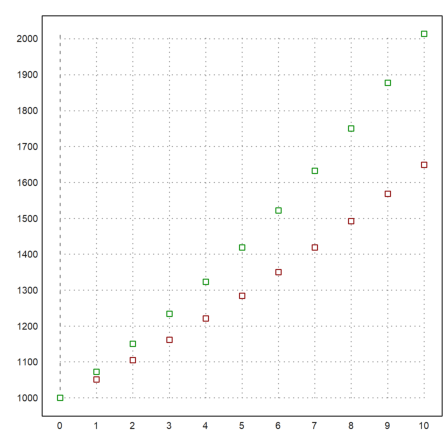
\includegraphics[keepaspectratio]{images/EMT4Statistika - Naila Khalidatus Salwa-049.png}}
\caption{images/EMT4Statistika\%20-\%20Naila\%20Khalidatus\%20Salwa-049.png}
\end{figure}

Ada beberapa cara yang lebih mendasar untuk membaca data dari file. Anda dapat membuka file dan membaca angka baris demi baris. Fungsi getvectorline() akan membaca angka dari sebuah baris data. Secara default, fungsi ini mengharapkan sebuah titik desimal. Tetapi fungsi ini juga dapat menggunakan koma desimal, jika Anda memanggil setdecimaldot(``,'') sebelum menggunakan fungsi ini.

Fungsi berikut adalah contoh untuk hal ini. Fungsi ini akan berhenti pada akhir file atau baris kosong.

\textgreater function myload (file) \ldots{}

\begin{verbatim}
open(file);
M=[];
repeat
   until eof();
   v=getvectorline(3);
   if length(v)>0 then M=M_v; else break; endif;
end;
return M;
close(file);
endfunction
\end{verbatim}

\textgreater myload(file)

\begin{verbatim}
  0.28316   0.40677   0.38266 
   0.8179   0.87308   0.97188 
  0.38798   0.45394   0.74251 
\end{verbatim}

Kita juga dapat membaca semua angka dalam file tersebut dengan getvector().

\textgreater open(file); v=getvector(10000); close(); redim(v{[}1:9{]},3,3)

\begin{verbatim}
  0.28316   0.40677   0.38266 
   0.8179   0.87308   0.97188 
  0.38798   0.45394   0.74251 
\end{verbatim}

Dengan demikian, sangat mudah untuk menyimpan vektor nilai, satu nilai di setiap baris dan membaca kembali vektor ini.

\textgreater v=random(1000); mean(v)

\begin{verbatim}
0.50418
\end{verbatim}

\textgreater writematrix(v',file); mean(readmatrix(file)')

\begin{verbatim}
0.50418
\end{verbatim}

\chapter{Menggunakan Tabel}\label{menggunakan-tabel}

Tabel dapat digunakan untuk membaca atau menulis data numerik. Sebagai contoh, kita menulis tabel dengan judul baris dan kolom ke file.

\textgreater file=``test.tab''; M=random(3,3); \ldots{}\\
\textgreater{} open(file,``w''); \ldots{}\\
\textgreater{} writetable(M,separator=``,'',labc={[}``one'',``two'',``three''{]}); \ldots{}\\
\textgreater{} close(); \ldots{}\\
\textgreater{} printfile(file)

\begin{verbatim}
one,two,three
      0.94,      0.26,      0.14
      0.98,      0.51,      0.95
      0.02,      0.23,      0.63
\end{verbatim}

Ini dapat diimpor ke Excel.

Untuk membaca file di EMT, kita menggunakan readtable().

\textgreater\{M,headings\}=readtable(file,\textgreater clabs); \ldots{}\\
\textgreater{} writetable(M,labc=headings)

\begin{verbatim}
       one       two     three
      0.94      0.26      0.14
      0.98      0.51      0.95
      0.02      0.23      0.63
\end{verbatim}

\chapter{Menganalisis Garis}\label{menganalisis-garis}

Pada subbab ini sering digunakan untuk memproses atau mengekstrak data dari teks yang berformat khusus, seperti data tabel dalam HTML.

Kita bahkan dapat mengevaluasi setiap garis dengan tangan. Misalkan, kita memiliki baris dengan format berikut.

\textgreater line=``2020-11-03,Tue,1'114.05''

\begin{verbatim}
2020-11-03,Tue,1'114.05
\end{verbatim}

Pertama, kita akan memisahkan string line menjadi bagian-bagian yang lebih kecil, yang dikenal sebagai ``token''.

\textgreater vt=strtokens(line)

\begin{verbatim}
2020-11-03
Tue
1'114.05
\end{verbatim}

Kemudian, kita dapat mengevaluasi setiap elemen garis dengan menggunakan evaluasi yang sesuai.

\textgreater day(vt{[}1{]}), \ldots{}\\
\textgreater{} indexof({[}``mon'',``tue'',``wed'',``thu'',``fri'',``sat'',``sun''{]},tolower(vt{[}2{]})), \ldots{}\\
\textgreater{} strrepl(vt{[}3{]},``''',``\,``)()

\begin{verbatim}
738162
2
1114.05
\end{verbatim}

Dengan menggunakan ekspresi reguler, Anda dapat mengekstrak hampir semua informasi dari sebuah baris data.

Anggaplah kita memiliki baris dokumen HTML berikut ini.

\textgreater line=``\textless tr\textgreater\textless td\textgreater1145.45\textless/td\textgreater\textless td\textgreater5.6\textless/td\textgreater\textless td\textgreater-4.5\textless/td\textgreater\textless tr\textgreater{}''

\begin{verbatim}
&lt;tr&gt;&lt;td&gt;1145.45&lt;/td&gt;&lt;td&gt;5.6&lt;/td&gt;&lt;td&gt;-4.5&lt;/td&gt;&lt;tr&gt;
\end{verbatim}

Untuk mengekstrak ini, kita menggunakan ekspresi reguler, yang mencari

\begin{itemize}
\item
  tanda kurung tutup \textgreater, untuk mengindikasikan bahwa kita akan mencari
\item
  awal dari elemen yang ada di dalam tag.
\item
  string apa pun yang tidak mengandung tanda kurung akan mencocokkan
\item
  elemen di dalam tag \textless td\textgreater,
\item
  tanda kurung pembuka dan penutup menggunakan solusi terpendek,
\item
  dengan tag pembuka (\textless td\textgreater) dan penutup (\textless/td\textgreater).
\item
  lagi-lagi string apa pun yang tidak mengandung tanda kurung, ini
\item
  akan menjamin bahwa kita akan mengambil isi yang relevan di dalam
\item
  tagnya.
\item
  dan tanda kurung pembuka \textless{} menandai bahwa ini adalah akhir dari tag
\item
  dan awal dari tag baru.
\end{itemize}

Ekspresi reguler agak sulit untuk dipelajari namun sangat kuat.

\textgreater\{pos,s,vt\}=strxfind(line,``\textgreater({[}\^{}\textless\textbackslash\textgreater{]}+)\textless.+?\textgreater({[}\^{}\textless\textbackslash\textgreater{]}+)\textless{}'');

Hasilnya adalah posisi kecocokan, string yang cocok, dan vektor string untuk sub-cocokan.

\textgreater for k=1:length(vt); vt\href{}{k}, end;

\begin{verbatim}
1145.5
5.6
\end{verbatim}

Berikut ini adalah fungsi yang membaca semua item numerik antara \textless td\textgreater{} dan \textless/td\textgreater.

\textgreater function readtd (line) \ldots{}

\begin{verbatim}
v=[]; cp=0;
repeat
   {pos,s,vt}=strxfind(line,"<td.*?>(.+?)</td>",cp);
   until pos==0;
   if length(vt)>0 then v=v|vt[1]; endif;
   cp=pos+strlen(s);
end;
return v;
endfunction
\end{verbatim}

\textgreater readtd(line+``\textless td\textgreater non-numerical\textless/td\textgreater{}'')

\begin{verbatim}
1145.45
5.6
-4.5
non-numerical
\end{verbatim}

\chapter{Membaca dari Web}\label{membaca-dari-web}

Sebuah situs web atau file dengan URL dapat dibuka di EMT dan dapat dibaca baris demi baris.

Dalam contoh, kami membaca versi saat ini dari situs EMT. Kami menggunakan ekspresi reguler untuk memindai ``Versi \ldots{}'' dalam judul.

\textgreater function readversion () \ldots{}

\begin{verbatim}
urlopen("http://www.euler-math-toolbox.de/Programs/Changes.html");
repeat
  until urleof();
  s=urlgetline();
  k=strfind(s,"Version ",1);
  if k>0 then substring(s,k,strfind(s,"<",k)-1), break; endif;
end;
urlclose();
endfunction
\end{verbatim}

\textgreater readversion

\begin{verbatim}
Version 2024-01-12
\end{verbatim}

\chapter{Input dan Output Variabel}\label{input-dan-output-variabel}

Kita dapat menulis variabel dalam bentuk definisi Euler ke file atau ke baris perintah.

\textgreater writevar(pi,``mypi'');

\begin{verbatim}
mypi = 3.141592653589793;
\end{verbatim}

Untuk pengujian, kami membuat file Euler di direktori kerja EMT.

\textgreater file=``test.e''; \ldots{}\\
\textgreater{} writevar(random(2,2),``M'',file); \ldots{}\\
\textgreater{} printfile(file,3)

\begin{verbatim}
M = [ ..
0.08620822118953746, 0.07470799579759112;
0.2945640487773084, 0.5524988979857445];
\end{verbatim}

Sekarang kita dapat memuat file tersebut. Ini akan mendefinisikan matriks M.

\textgreater load(file); show M,

\begin{verbatim}
M = 
 0.086208  0.074708 
  0.29456    0.5525 
\end{verbatim}

Sebagai catatan, jika writevar() digunakan pada sebuah variabel, maka ia akan mencetak definisi variabel dengan nama variabel tersebut.

\textgreater writevar(M); writevar(inch\$)

\begin{verbatim}
M = [ ..
0.08620822118953746, 0.07470799579759112;
0.2945640487773084, 0.5524988979857445];
inch$ = 0.0254;
\end{verbatim}

Kita juga dapat membuka file baru atau menambahkan ke file yang sudah ada. Dalam contoh ini, kami menambahkan ke file yang telah dibuat sebelumnya.

\textgreater open(file,``a''); \ldots{}\\
\textgreater{} writevar(random(2,2),``M1''); \ldots{}\\
\textgreater{} writevar(random(3,1),``M2''); \ldots{}\\
\textgreater{} close();

\textgreater load(file); show M1; show M2;

\begin{verbatim}
M1 = 
  0.84971   0.60496 
  0.40399   0.66191 
M2 = 
  0.70558 
  0.96423 
  0.54976 
\end{verbatim}

Untuk menghapus file, gunakan fileremove().

\textgreater fileremove(file);

Vektor baris dalam file tidak memerlukan koma, jika setiap angka berada di baris baru. Mari kita buat file seperti itu, dengan menulis setiap baris satu per satu dengan writeln().

\textgreater open(file,``w''); writeln(``M = {[}''); \ldots{}\\
\textgreater{} for i=1 to 5; writeln(''\,''+random()); end; \ldots{}\\
\textgreater{} writeln(''{]};''); close(); \ldots{}\\
\textgreater{} printfile(file)

\begin{verbatim}
M = [
0.448345488454
0.28912147627
0.997745871455
0.548465389581
0.491125845232
];
\end{verbatim}

\textgreater load(file); M

\begin{verbatim}
[0.44835,  0.28912,  0.99775,  0.54847,  0.49113]
\end{verbatim}

LATIHAN

\begin{center}\rule{0.5\linewidth}{0.5pt}\end{center}

\begin{enumerate}
\def\labelenumi{\arabic{enumi}.}
\tightlist
\item
  Misalkan vektor x={[}2, 4, 6, 8, 10{]}
\end{enumerate}

\begin{enumerate}
\def\labelenumi{\alph{enumi}.}
\item
  Buatkan vektor yang menggabungkan vektor x, angka 0, dan vektor x lagi
\item
  Tentukan apakah setiap elemen vektor x lebih besar dari 5! (hasil logika 1 untuk benar dan 0 untuk salah)
\end{enumerate}

\textgreater x := {[}2,4,6,8,10{]}; {[}x,0,x{]}

\begin{verbatim}
[2,  4,  6,  8,  10,  0,  2,  4,  6,  8,  10]
\end{verbatim}

\textgreater x\textgreater5, \%*x

\begin{verbatim}
[0,  0,  1,  1,  1]
[0,  0,  6,  8,  10]
\end{verbatim}

\begin{enumerate}
\def\labelenumi{\arabic{enumi}.}
\setcounter{enumi}{1}
\tightlist
\item
  Tentukan matriks X dengan elemen-elemen yang berurutan dari 1 hingga 20 dan susunlah elemen tersebut menjadi matriks berukuran 5x4.
\end{enumerate}

\textgreater shortformat; X=redim(1:20,5,4)

\begin{verbatim}
        1         2         3         4 
        5         6         7         8 
        9        10        11        12 
       13        14        15        16 
       17        18        19        20 
\end{verbatim}

\begin{enumerate}
\def\labelenumi{\arabic{enumi}.}
\setcounter{enumi}{2}
\tightlist
\item
  Seorang analis memiliki data penjualan harian selama 5 hari (150,200,250,300,350) yang disimpan dalam bentuk vektor sebagai berikut:
\end{enumerate}

\begin{enumerate}
\def\labelenumi{\alph{enumi}.}
\item
  Mean (rata-rata)
\item
  Deviasi standar
\end{enumerate}

\textgreater penjualan={[}150,200,250,300,350{]}

\begin{verbatim}
[150,  200,  250,  300,  350]
\end{verbatim}

\textgreater filename=``penjulan.dat'';

\textgreater writematrix(penjualan',filename)

\textgreater penjualan=readmatrix(filename)'

\begin{verbatim}
[150,  200,  250,  300,  350]
\end{verbatim}

\textgreater mean(penjualan)

\begin{verbatim}
250
\end{verbatim}

\textgreater dev(penjualan)

\begin{verbatim}
79.057
\end{verbatim}

\textgreater{}

\begin{enumerate}
\def\labelenumi{\arabic{enumi}.}
\setcounter{enumi}{3}
\tightlist
\item
  Buat fungsi yang membuka URL
\end{enumerate}

``https://en.wikipedia.org/wiki/Euler\_(software)''

dan mencari kata ``Versi'' di dalam URL tersebut, dan tampilkan hasilnya

\textgreater function readversion () \ldots{}

\begin{verbatim}
urlopen("https://en.wikipedia.org/wiki/Euler_(software)");
repeat
  until urleof();
  s=urlgetline();
  k=strfind(s,"Version ",1);
  if k>0 then substring(s,k,strfind(s,"<",k)-1), break; endif;
end;
urlclose();
endfunction
\end{verbatim}

\textgreater readversion

\begin{verbatim}
Version 2022-05-18"
\end{verbatim}

\begin{enumerate}
\def\labelenumi{\arabic{enumi}.}
\setcounter{enumi}{4}
\tightlist
\item
  Cari apakah ada hubungan antara jenis kelamin dan kecenderungan seseorang untuk memilih warna merah atau biru. Berikut adalah tabel kontingensi:
\end{enumerate}

\textgreater A={[}10,20;15,5{]};\ldots{}\\
\textgreater{} writetable(A,wc=2,labr={[}``m'',``f''{]},labc={[}``merah'',``biru''{]})

\begin{verbatim}
   merah biru
 m    10   20
 f    15    5
\end{verbatim}

\textgreater tabletest(A)

\begin{verbatim}
0.00389241712278
\end{verbatim}

Hasilnya terlalu kecil untuk menolak independensi. Jadi kita dapat mengatakan, jika jenis kelamin berhubungan dengan kecenderungan seseorang untuk memilih warna merah atau biru.

Berikut ini adalah tabel yang diharapkan,

\textgreater writetable(expectedtable(A),wc=2,labr={[}``m'',``f''{]},labc={[}``merah'',``biru''{]})

\begin{verbatim}
   merah biru
 m    15   15
 f    10   10
\end{verbatim}

\textgreater contingency(A)

\begin{verbatim}
0.534522483825
\end{verbatim}

Kita dapat menghitung koefisien kontingensi terkoreksi. Karena koefisien ini cukup jauh dengan 0, kita dapat menyimpulkan bahwa kecenderungan memilih warna biru dan merah bergantung pada jenis kelamin.

\textgreater{}

\backmatter
\end{document}
